%%%%%%%%%%%%%%%%%%%%%%%%%%%%%%%%%%%%%%%%%
% This report has been adapted from the following template:
% The Legrand Orange Book
% LaTeX Template
% Version 2.4 (26/09/2018)
%
% This template was downloaded from:
% http://www.LaTeXTemplates.com
%
% Original author:
% Mathias Legrand (legrand.mathias@gmail.com) with modifications by:
% Vel (vel@latextemplates.com)
%
% License:
% CC BY-NC-SA 3.0 (http://creativecommons.org/licenses/by-nc-sa/3.0/)
%
% Some changes made to the template:
% We use natbib for citations, and this significantly changes the Bibliography page
% We also change the colors and images used in the chapter headers and so on.
%
%
% This template also uses a number of packages which may need to be
% updated to the newest versions for the template to compile. It is strongly
% recommended you update your LaTeX distribution if you have any
% compilation errors.
%
% Important note:
% Chapter heading images should have a 2:1 width:height ratio,
% e.g. 920px width and 460px height.
%
%%%%%%%%%%%%%%%%%%%%%%%%%%%%%%%%%%%%%%%%%

%----------------------------------------------------------------------------------------
%	PACKAGES AND OTHER DOCUMENT CONFIGURATIONS
%----------------------------------------------------------------------------------------

\documentclass[11pt]{book} % Default font size
\usepackage{blindtext}
\usepackage{lipsum}
\usepackage{textcomp}
\usepackage{gensymb}
\usepackage{mathtools}
% \usepackage{subfigure}
\usepackage{titling}
\usepackage{authblk}
\usepackage{eso-pic}
\usepackage[nottoc]{tocbibind}
\usepackage{natbib}
\usepackage{aas_macros}
\usepackage[outputdir=cache]{minted}
\usepackage{listings}
\usepackage{xcolor}
\usepackage{graphics}
\usepackage{float}
\usepackage{wrapfig}
\usepackage{amsmath}
\usepackage{amssymb}
\usepackage{units}
\usepackage[utf8]{inputenc}
\usepackage{subcaption}
\usepackage[export]{adjustbox}
\usepackage{url}
\usepackage{hyperref}
\usepackage{xcolor}
% \usepackage{wasysym}
% \usepackage{marvosym}
% \usepackage{gensymb}

\definecolor{codegreen}{rgb}{0,0.6,0}
\definecolor{codegray}{rgb}{0.5,0.5,0.5}
\definecolor{codepurple}{rgb}{0.58,0,0.82}
\definecolor{backcolour}{rgb}{0.95,0.95,0.92}

\lstdefinestyle{mystyle}{
    backgroundcolor=\color{backcolour},   
    commentstyle=\color{codegreen},
    keywordstyle=\color{magenta},
    numberstyle=\tiny\color{codegray},
    stringstyle=\color{codepurple},
    basicstyle=\ttfamily,
    \lst@ifdisplaystyle\scriptsize\fi,
    breakatwhitespace=false,         
    breaklines=true,                 
    captionpos=b,                    
    keepspaces=true,                 
    numbers=left,                    
    numbersep=5pt,                  
    showspaces=false,                
    showstringspaces=false,
    showtabs=false,                  
    tabsize=2
}

\lstset{style=mystyle}

%% THEME
%%%%%%%%%%%%%%%%%%%%%%%%%%%%%%%%%%%%%%%%%
% The Legrand Orange Book
% Structural Definitions File
% Version 2.1 (26/09/2018)
%
% Original author:
% Mathias Legrand (legrand.mathias@gmail.com) with modifications by:
% Vel (vel@latextemplates.com)
% 
% This file was downloaded from:
% http://www.LaTeXTemplates.com
%
% License:
% CC BY-NC-SA 3.0 (http://creativecommons.org/licenses/by-nc-sa/3.0/)
%
%%%%%%%%%%%%%%%%%%%%%%%%%%%%%%%%%%%%%%%%%

%----------------------------------------------------------------------------------------
%	VARIOUS REQUIRED PACKAGES AND CONFIGURATIONS
%----------------------------------------------------------------------------------------

\usepackage{graphicx} % Required for including pictures
\graphicspath{{Pictures/}} % Specifies the directory where pictures are stored

\usepackage{lipsum} % Inserts dummy text

\usepackage{tikz} % Required for drawing custom shapes

\usepackage[english]{babel} % English language/hyphenation

\usepackage{enumitem} % Customize lists
\setlist{nolistsep} % Reduce spacing between bullet points and numbered lists

\usepackage{booktabs} % Required for nicer horizontal rules in tables

\usepackage{xcolor} % Required for specifying colors by name
\definecolor{theme}{RGB}{243,102,25} % Define the orange color used for highlighting throughout the book


%----------------------------------------------------------------------------------------
%	MARGINS
%----------------------------------------------------------------------------------------

\usepackage{geometry} % Required for adjusting page dimensions and margins

\geometry{
	paper=a4paper, % Paper size, change to letterpaper for US letter size
	top=3cm, % Top margin
	bottom=3cm, % Bottom margin
	left=3cm, % Left margin
	right=3cm, % Right margin
	headheight=14pt, % Header height
	footskip=1.4cm, % Space from the bottom margin to the baseline of the footer
	headsep=10pt, % Space from the top margin to the baseline of the header
	%showframe, % Uncomment to show how the type block is set on the page
}

%----------------------------------------------------------------------------------------
%	FONTS
%----------------------------------------------------------------------------------------

\usepackage{avant} % Use the Avantgarde font for headings
%\usepackage{times} % Use the Times font for headings
\usepackage{mathptmx} % Use the Adobe Times Roman as the default text font together with math symbols from the Sym­bol, Chancery and Com­puter Modern fonts

\usepackage{microtype} % Slightly tweak font spacing for aesthetics
\usepackage[utf8]{inputenc} % Required for including letters with accents
\usepackage[T1]{fontenc} % Use 8-bit encoding that has 256 glyphs

%----------------------------------------------------------------------------------------
%	BIBLIOGRAPHY AND INDEX
%----------------------------------------------------------------------------------------

%\usepackage[style=numeric,citestyle=numeric,sorting=nyt,sortcites=true,autopunct=true,babel=hyphen,hyperref=true,abbreviate=false,backref=true,backend=biber]{biblatex}
%\addbibresource{bibliography.bib} % BibTeX bibliography file
%\defbibheading{bibempty}{}
\usepackage{natbib}


\usepackage{calc} % For simpler calculation - used for spacing the index letter headings correctly
\usepackage{makeidx} % Required to make an index
\makeindex % Tells LaTeX to create the files required for indexing

%----------------------------------------------------------------------------------------
%	MAIN TABLE OF CONTENTS
%----------------------------------------------------------------------------------------

\usepackage{titletoc} % Required for manipulating the table of contents

\contentsmargin{0cm} % Removes the default margin

% Part text styling (this is mostly taken care of in the PART HEADINGS section of this file)
\titlecontents{part}
	[0cm] % Left indentation
	{\addvspace{20pt}\bfseries} % Spacing and font options for parts
	{}
	{}
	{}

% Chapter text styling
\titlecontents{chapter}
	[1.25cm] % Left indentation
	{\addvspace{12pt}\large\sffamily\bfseries} % Spacing and font options for chapters
	{\color{theme!60}\contentslabel[\Large\thecontentslabel]{1.25cm}\color{theme}} % Formatting of numbered sections of this type
	{\color{theme}} % Formatting of numberless sections of this type
	{\color{theme!60}\normalsize\;\titlerule*[.5pc]{.}\;\thecontentspage} % Formatting of the filler to the right of the heading and the page number

% Section text styling
\titlecontents{section}
	[1.25cm] % Left indentation
	{\addvspace{3pt}\sffamily\bfseries} % Spacing and font options for sections
	{\contentslabel[\thecontentslabel]{1.25cm}} % Formatting of numbered sections of this type
	{} % Formatting of numberless sections of this type
	{\hfill\color{black}\thecontentspage} % Formatting of the filler to the right of the heading and the page number

% Subsection text styling
\titlecontents{subsection}
	[1.25cm] % Left indentation
	{\addvspace{1pt}\sffamily\small} % Spacing and font options for subsections
	{\contentslabel[\thecontentslabel]{1.25cm}} % Formatting of numbered sections of this type
	{} % Formatting of numberless sections of this type
	{\ \titlerule*[.5pc]{.}\;\thecontentspage} % Formatting of the filler to the right of the heading and the page number

% Figure text styling
\titlecontents{figure}
	[1.25cm] % Left indentation
	{\addvspace{1pt}\sffamily\small} % Spacing and font options for figures
	{\thecontentslabel\hspace*{1em}} % Formatting of numbered sections of this type
	{} % Formatting of numberless sections of this type
	{\ \titlerule*[.5pc]{.}\;\thecontentspage} % Formatting of the filler to the right of the heading and the page number

% Table text styling
\titlecontents{table}
	[1.25cm] % Left indentation
	{\addvspace{1pt}\sffamily\small} % Spacing and font options for tables
	{\thecontentslabel\hspace*{1em}} % Formatting of numbered sections of this type
	{} % Formatting of numberless sections of this type
	{\ \titlerule*[.5pc]{.}\;\thecontentspage} % Formatting of the filler to the right of the heading and the page number

%----------------------------------------------------------------------------------------
%	MINI TABLE OF CONTENTS IN PART HEADS
%----------------------------------------------------------------------------------------

% Chapter text styling
\titlecontents{lchapter}
	[0em] % Left indentation
	{\addvspace{15pt}\large\sffamily\bfseries} % Spacing and font options for chapters
	{\color{theme}\contentslabel[\Large\thecontentslabel]{1.25cm}\color{theme}} % Chapter number
	{}  
	{\color{theme}\normalsize\sffamily\bfseries\;\titlerule*[.5pc]{.}\;\thecontentspage} % Page number

% Section text styling
\titlecontents{lsection}
	[0em] % Left indentation
	{\sffamily\small} % Spacing and font options for sections
	{\contentslabel[\thecontentslabel]{1.25cm}} % Section number
	{}
	{}

% Subsection text styling (note these aren't shown by default, display them by searchings this file for tocdepth and reading the commented text)
\titlecontents{lsubsection}
	[.5em] % Left indentation
	{\sffamily\footnotesize} % Spacing and font options for subsections
	{\contentslabel[\thecontentslabel]{1.25cm}}
	{}
	{}

%----------------------------------------------------------------------------------------
%	HEADERS AND FOOTERS
%----------------------------------------------------------------------------------------

\usepackage{fancyhdr} % Required for header and footer configuration

\pagestyle{fancy} % Enable the custom headers and footers

\renewcommand{\chaptermark}[1]{\markboth{\sffamily\normalsize\bfseries\chaptername\ \thechapter.\ #1}{}} % Styling for the current chapter in the header
\renewcommand{\sectionmark}[1]{\markright{\sffamily\normalsize\thesection\hspace{5pt}#1}{}} % Styling for the current section in the header

\fancyhf{} % Clear default headers and footers
\fancyhead[LE,RO]{\sffamily\normalsize\thepage} % Styling for the page number in the header
\fancyhead[LO]{\rightmark} % Print the nearest section name on the left side of odd pages
\fancyhead[RE]{\leftmark} % Print the current chapter name on the right side of even pages
%\fancyfoot[C]{\thepage} % Uncomment to include a footer

\renewcommand{\headrulewidth}{0.5pt} % Thickness of the rule under the header

\fancypagestyle{plain}{% Style for when a plain pagestyle is specified
	\fancyhead{}\renewcommand{\headrulewidth}{0pt}%
}

% Removes the header from odd empty pages at the end of chapters
\makeatletter
\renewcommand{\cleardoublepage}{
\clearpage\ifodd\c@page\else
\hbox{}
% \vspace*{\fill}
\thispagestyle{empty}
% \newpage
\fi}

%----------------------------------------------------------------------------------------
%	THEOREM STYLES
%----------------------------------------------------------------------------------------

\usepackage{amsmath,amsfonts,amssymb,amsthm} % For math equations, theorems, symbols, etc

\newcommand{\intoo}[2]{\mathopen{]}#1\,;#2\mathclose{[}}
\newcommand{\ud}{\mathop{\mathrm{{}d}}\mathopen{}}
\newcommand{\intff}[2]{\mathopen{[}#1\,;#2\mathclose{]}}
\renewcommand{\qedsymbol}{$\blacksquare$}
\newtheorem{notation}{Notation}[chapter]

% Boxed/framed environments
\newtheoremstyle{themenumbox}% Theorem style name
{0pt}% Space above
{0pt}% Space below
{\normalfont}% Body font
{}% Indent amount
{\small\bf\sffamily\color{theme}}% Theorem head font
{\;}% Punctuation after theorem head
{0.25em}% Space after theorem head
{\small\sffamily\color{theme}\thmname{#1}\nobreakspace\thmnumber{\@ifnotempty{#1}{}\@upn{#2}}% Theorem text (e.g. Theorem 2.1)
\thmnote{\nobreakspace\the\thm@notefont\sffamily\bfseries\color{black}---\nobreakspace#3.}} % Optional theorem note

\newtheoremstyle{blacknumex}% Theorem style name
{5pt}% Space above
{5pt}% Space below
{\normalfont}% Body font
{} % Indent amount
{\small\bf\sffamily}% Theorem head font
{\;}% Punctuation after theorem head
{0.25em}% Space after theorem head
{\small\sffamily{\tiny\ensuremath{\blacksquare}}\nobreakspace\thmname{#1}\nobreakspace\thmnumber{\@ifnotempty{#1}{}\@upn{#2}}% Theorem text (e.g. Theorem 2.1)
\thmnote{\nobreakspace\the\thm@notefont\sffamily\bfseries---\nobreakspace#3.}}% Optional theorem note

\newtheoremstyle{blacknumbox} % Theorem style name
{0pt}% Space above
{0pt}% Space below
{\normalfont}% Body font
{}% Indent amount
{\small\bf\sffamily}% Theorem head font
{\;}% Punctuation after theorem head
{0.25em}% Space after theorem head
{\small\sffamily\thmname{#1}\nobreakspace\thmnumber{\@ifnotempty{#1}{}\@upn{#2}}% Theorem text (e.g. Theorem 2.1)
\thmnote{\nobreakspace\the\thm@notefont\sffamily\bfseries---\nobreakspace#3.}}% Optional theorem note

% Non-boxed/non-framed environments
\newtheoremstyle{themenum}% Theorem style name
{5pt}% Space above
{5pt}% Space below
{\normalfont}% Body font
{}% Indent amount
{\small\bf\sffamily\color{theme}}% Theorem head font
{\;}% Punctuation after theorem head
{0.25em}% Space after theorem head
{\small\sffamily\color{theme}\thmname{#1}\nobreakspace\thmnumber{\@ifnotempty{#1}{}\@upn{#2}}% Theorem text (e.g. Theorem 2.1)
\thmnote{\nobreakspace\the\thm@notefont\sffamily\bfseries\color{black}---\nobreakspace#3.}} % Optional theorem note
\makeatother

% Defines the theorem text style for each type of theorem to one of the three styles above
\newcounter{dummy} 
\numberwithin{dummy}{section}
\theoremstyle{themenumbox}
\newtheorem{theoremeT}[dummy]{Theorem}
\newtheorem{problem}{Problem}[chapter]
\newtheorem{exerciseT}{Exercise}[chapter]
\theoremstyle{blacknumex}
\newtheorem{exampleT}{Example}[chapter]
\theoremstyle{blacknumbox}
\newtheorem{vocabulary}{Vocabulary}[chapter]
\newtheorem{definitionT}{Definition}[section]
\newtheorem{corollaryT}[dummy]{Corollary}
\theoremstyle{themenum}
\newtheorem{proposition}[dummy]{Proposition}

%----------------------------------------------------------------------------------------
%	DEFINITION OF COLORED BOXES
%----------------------------------------------------------------------------------------

\RequirePackage[framemethod=default]{mdframed} % Required for creating the theorem, definition, exercise and corollary boxes

% Theorem box
\newmdenv[skipabove=7pt,
skipbelow=7pt,
backgroundcolor=black!15,
linecolor=theme,
innerleftmargin=5pt,
innerrightmargin=5pt,
innertopmargin=5pt,
leftmargin=0cm,
rightmargin=0cm,
innerbottommargin=5pt]{tBox}

% Exercise box	  
\newmdenv[skipabove=7pt,
skipbelow=7pt,
rightline=false,
leftline=true,
topline=false,
bottomline=false,
backgroundcolor=theme!20,
linecolor=theme,
innerleftmargin=5pt,
innerrightmargin=5pt,
innertopmargin=5pt,
innerbottommargin=5pt,
leftmargin=0cm,
rightmargin=0cm,
linewidth=4pt]{eBox}	

% Definition box
\newmdenv[skipabove=7pt,
skipbelow=7pt,
rightline=false,
leftline=true,
topline=false,
bottomline=false,
linecolor=theme,
innerleftmargin=5pt,
innerrightmargin=5pt,
innertopmargin=0pt,
leftmargin=0cm,
rightmargin=0cm,
linewidth=4pt,
innerbottommargin=0pt]{dBox}	

% Corollary box
\newmdenv[skipabove=7pt,
skipbelow=7pt,
rightline=false,
leftline=true,
topline=false,
bottomline=false,
linecolor=gray,
backgroundbicolor=black!5,
innerleftmargin=5pt,
innerrightmargin=5pt,
innertopmargin=5pt,
leftmargin=0cm,
rightmargin=0cm,
linewidth=4pt,
innerbottommargin=5pt]{cBox}

% Creates an environment for each type of theorem and assigns it a theorem text style from the "Theorem Styles" section above and a colored box from above
\newenvironment{theorem}{\begin{tBox}\begin{theoremeT}}{\end{theoremeT}\end{tBox}}
\newenvironment{exercise}{\begin{eBox}\begin{exerciseT}}{\hfill{\color{theme}\tiny\ensuremath{\blacksquare}}\end{exerciseT}\end{eBox}}				  
\newenvironment{definition}{\begin{dBox}\begin{definitionT}}{\end{definitionT}\end{dBox}}	
\newenvironment{example}{\begin{exampleT}}{\hfill{\tiny\ensuremath{\blacksquare}}\end{exampleT}}		
\newenvironment{corollary}{\begin{cBox}\begin{corollaryT}}{\end{corollaryT}\end{cBox}}	

%----------------------------------------------------------------------------------------
%	REMARK ENVIRONMENT
%----------------------------------------------------------------------------------------

\newenvironment{remark}{\par\vspace{10pt}\small % Vertical white space above the remark and smaller font size
\begin{list}{}{
\leftmargin=35pt % Indentation on the left
\rightmargin=25pt}\item\ignorespaces % Indentation on the right
\makebox[-2.5pt]{\begin{tikzpicture}[overlay]
\node[draw=theme!60,line width=1pt,circle,fill=theme!25,font=\sffamily\bfseries,inner sep=2pt,outer sep=0pt] at (-15pt,0pt){\textcolor{theme}{R}};\end{tikzpicture}} % Orange R in a circle
\advance\baselineskip -1pt}{\end{list}\vskip5pt} % Tighter line spacing and white space after remark

%----------------------------------------------------------------------------------------
%	SECTION NUMBERING IN THE MARGIN
%----------------------------------------------------------------------------------------

\makeatletter
\renewcommand{\@seccntformat}[1]{\llap{\textcolor{theme}{\csname the#1\endcsname}\hspace{1em}}}                    
\renewcommand{\section}{\@startsection{section}{1}{\z@}
{-4ex \@plus -1ex \@minus -.4ex}
{1ex \@plus.2ex }
{\normalfont\large\sffamily\bfseries}}
\renewcommand{\subsection}{\@startsection {subsection}{2}{\z@}
{-3ex \@plus -0.1ex \@minus -.4ex}
{0.5ex \@plus.2ex }
{\normalfont\sffamily\bfseries}}
\renewcommand{\subsubsection}{\@startsection {subsubsection}{3}{\z@}
{-2ex \@plus -0.1ex \@minus -.2ex}
{.2ex \@plus.2ex }
{\normalfont\small\sffamily\bfseries}}                        
\renewcommand\paragraph{\@startsection{paragraph}{4}{\z@}
{-2ex \@plus-.2ex \@minus .2ex}
{.1ex}
{\normalfont\small\sffamily\bfseries}}

%----------------------------------------------------------------------------------------
%	PART HEADINGS
%----------------------------------------------------------------------------------------

% Numbered part in the table of contents
\newcommand{\@mypartnumtocformat}[2]{%
	\setlength\fboxsep{0pt}%
	\noindent\colorbox{theme!20}{\strut\parbox[c][.7cm]{\ecart}{\color{theme!90}\Large\sffamily\bfseries\centering#1}}\hskip\esp\colorbox{theme!40}{\strut\parbox[c][.7cm]{\linewidth-\ecart-\esp}{\Large\sffamily\centering#2}}%
}

% Unnumbered part in the table of contents
\newcommand{\@myparttocformat}[1]{%
	\setlength\fboxsep{0pt}%
	\noindent\colorbox{theme!40}{\strut\parbox[c][.7cm]{\linewidth}{\Large\sffamily\centering#1}}%
}

\newlength\esp
\setlength\esp{4pt}
\newlength\ecart
\setlength\ecart{1.2cm-\esp}
\newcommand{\thepartimage}{}%
\newcommand{\partimage}[1]{\renewcommand{\thepartimage}{#1}}%
\def\@part[#1]#2{%
\ifnum \c@secnumdepth >-2\relax%
\refstepcounter{part}%
\addcontentsline{toc}{part}{\texorpdfstring{\protect\@mypartnumtocformat{\thepart}{#1}}{\partname~\thepart\ ---\ #1}}
\else%
\addcontentsline{toc}{part}{\texorpdfstring{\protect\@myparttocformat{#1}}{#1}}%
\fi%
\startcontents%
\markboth{}{}%
{\thispagestyle{empty}%
\begin{tikzpicture}[remember picture,overlay]%
\node at (current page.north west){\begin{tikzpicture}[remember picture,overlay]%	
\fill[theme!20](0cm,0cm) rectangle (\paperwidth,-\paperheight);
\node[anchor=north] at (4cm,-3.25cm){\color{theme!80}\fontsize{220}{100}\sffamily\bfseries\thepart}; 
\node[anchor=south east] at (\paperwidth-1cm,-\paperheight+1cm){\parbox[t][][t]{8.5cm}{
\printcontents{l}{0}{\setcounter{tocdepth}{1}}% The depth to which the Part mini table of contents displays headings; 0 for chapters only, 1 for chapters and sections and 2 for chapters, sections and subsections
}};
\node[anchor=north east] at (\paperwidth-1.5cm,-3.25cm){\parbox[t][][t]{15cm}{\strut\raggedleft\color{theme!80}\fontsize{30}{30}\sffamily\bfseries#2}};
\end{tikzpicture}};
\end{tikzpicture}}%
\@endpart}
\def\@spart#1{%
\startcontents%
\phantomsection
{\thispagestyle{empty}%
\begin{tikzpicture}[remember picture,overlay]%
\node at (current page.north west){\begin{tikzpicture}[remember picture,overlay]%	
\fill[theme!20](0cm,0cm) rectangle (\paperwidth,-\paperheight);
\node[anchor=north east] at (\paperwidth-1.5cm,-3.25cm){\parbox[t][][t]{15cm}{\strut\raggedleft\color{white}\fontsize{30}{30}\sffamily\bfseries#1}};
\end{tikzpicture}};
\end{tikzpicture}}
\addcontentsline{toc}{part}{\texorpdfstring{%
\setlength\fboxsep{0pt}%
\noindent\protect\colorbox{theme!40}{\strut\protect\parbox[c][.7cm]{\linewidth}{\Large\sffamily\protect\centering #1\quad\mbox{}}}}{#1}}%
\@endpart}
\def\@endpart{\vfil
\newpage
\if@twoside
\if@openright
\null
\thispagestyle{empty}%
\newpage
\fi
\fi
\if@tempswa
\twocolumn
\fi}

%----------------------------------------------------------------------------------------
%	CHAPTER HEADINGS
%----------------------------------------------------------------------------------------

% A switch to conditionally include a picture, implemented by Christian Hupfer
\newif\ifusechapterimage
\usechapterimagetrue
\newcommand{\thechapterimage}{}%
\newcommand{\chapterimage}[1]{\ifusechapterimage\renewcommand{\thechapterimage}{#1}\fi}%
\newcommand{\autodot}{.}
\def\@makechapterhead#1{%
{\parindent \z@ \raggedright \normalfont
\ifnum \c@secnumdepth >\m@ne
\if@mainmatter
\begin{tikzpicture}[remember picture,overlay]
\node at (current page.north west)
{\begin{tikzpicture}[remember picture,overlay]
\node[anchor=north west,inner sep=0pt] at (0,0) {\ifusechapterimage\includegraphics[width=\paperwidth]{\thechapterimage}\fi};
\draw[anchor=west] (\Gm@lmargin,-9cm) node [line width=2pt,rounded corners=15pt,draw=theme,fill=white,fill opacity=0.5,inner sep=15pt]{\strut\makebox[22cm]{}};
\draw[anchor=west] (\Gm@lmargin+.3cm,-9cm) node {\huge\sffamily\bfseries\color{black}\thechapter\autodot~#1\strut};
\end{tikzpicture}};
\end{tikzpicture}
\else
\begin{tikzpicture}[remember picture,overlay]
\node at (current page.north west)
{\begin{tikzpicture}[remember picture,overlay]
\node[anchor=north west,inner sep=0pt] at (0,0) {\ifusechapterimage\includegraphics[width=\paperwidth]{\thechapterimage}\fi};
\draw[anchor=west] (\Gm@lmargin,-9cm) node [line width=2pt,rounded corners=15pt,draw=theme,fill=white,fill opacity=0.5,inner sep=15pt]{\strut\makebox[22cm]{}};
\draw[anchor=west] (\Gm@lmargin+.3cm,-9cm) node {\huge\sffamily\bfseries\color{black}#1\strut};
\end{tikzpicture}};
\end{tikzpicture}
\fi\fi\par\vspace*{270\p@}}}

%-------------------------------------------

\def\@makeschapterhead#1{%
\begin{tikzpicture}[remember picture,overlay]
\node at (current page.north west)
{\begin{tikzpicture}[remember picture,overlay]
\node[anchor=north west,inner sep=0pt] at (0,0) {\ifusechapterimage\includegraphics[width=\paperwidth]{\thechapterimage}\fi};
\draw[anchor=west] (\Gm@lmargin,-9cm) node [line width=2pt,rounded corners=15pt,draw=theme,fill=white,fill opacity=0.5,inner sep=15pt]{\strut\makebox[22cm]{}};
\draw[anchor=west] (\Gm@lmargin+.3cm,-9cm) node {\huge\sffamily\bfseries\color{black}#1\strut};
\end{tikzpicture}};
\end{tikzpicture}
\par\vspace*{270\p@}}
\makeatother

%----------------------------------------------------------------------------------------
%	LINKS
%----------------------------------------------------------------------------------------

\usepackage{hyperref}
\hypersetup{hidelinks,colorlinks=true,breaklinks=true,urlcolor=theme,bookmarks=true,bookmarksopen=false,filecolor=theme, linkcolor=theme}

\usepackage{bookmark}
\bookmarksetup{
open,
numbered,
addtohook={%
\ifnum\bookmarkget{level}=0 % chapter
\bookmarksetup{bold}%
\fi
\ifnum\bookmarkget{level}=-1 % part
\bookmarksetup{color=theme,bold}%
\fi
}
}
 % Insert the commands.tex file which contains the majority of the structure behind the template

\definecolor{theme}{RGB}{76,139,245} % Redefine the color used for highlighting throughout the book. 

\renewcommand{\familydefault}{\sfdefault}

%\hypersetup{pdftitle={Title},pdfauthor={Author}} % Uncomment and fill out to include PDF metadata for the author and title of the book

%----------------------------------------------------------------------------------------

%% TITLE 
\title{\color{white}
	{\LARGE\sffamily\textsc{\color{black}Krittika Summer Projects 2023}}\\
	\normalfont\fontsize{35}{35}\selectfont
	\textbf{\color{black} Faintest of the Brightest}}

%% AUTHORS and AFFILIATIONS
\author[1,2]{\color{black}Ravi Kumar}
\author[1,2,3]{\color{black}Gaurav Waratkar}
\author[2,3]{\color{black}Meghna Dixit}


\setlength{\affilsep}{3em}
% Check your affiliations
\affil[1]{\protect\raggedright\normalfont\fontsize{10}{0}\selectfont Krittika - The Astronomy Club of IIT Bombay, Powai, Mumbai - 400076, India}
\affil[2]{Indian Institute of Technology Bombay, Mumbai - 400076, India}
\affil[3]{Mentor for the Project}


\date{}


\begin{document}
\makeatletter
\newcommand{\printauthorlist}{
    \begin{center}
		\expandafter\let\csname textsuperscript \endcsname\@gobble % Remove \textsuperscript 
		\AB@authlist% Print list
	\end{center}
}
\makeatother

%----------------------------------------------------------------------------------------
%	TITLE PAGE
%----------------------------------------------------------------------------------------

\begin{titlepage}
	\begingroup
	\thispagestyle{empty}
        \begin{center}
	\AddToShipoutPicture*{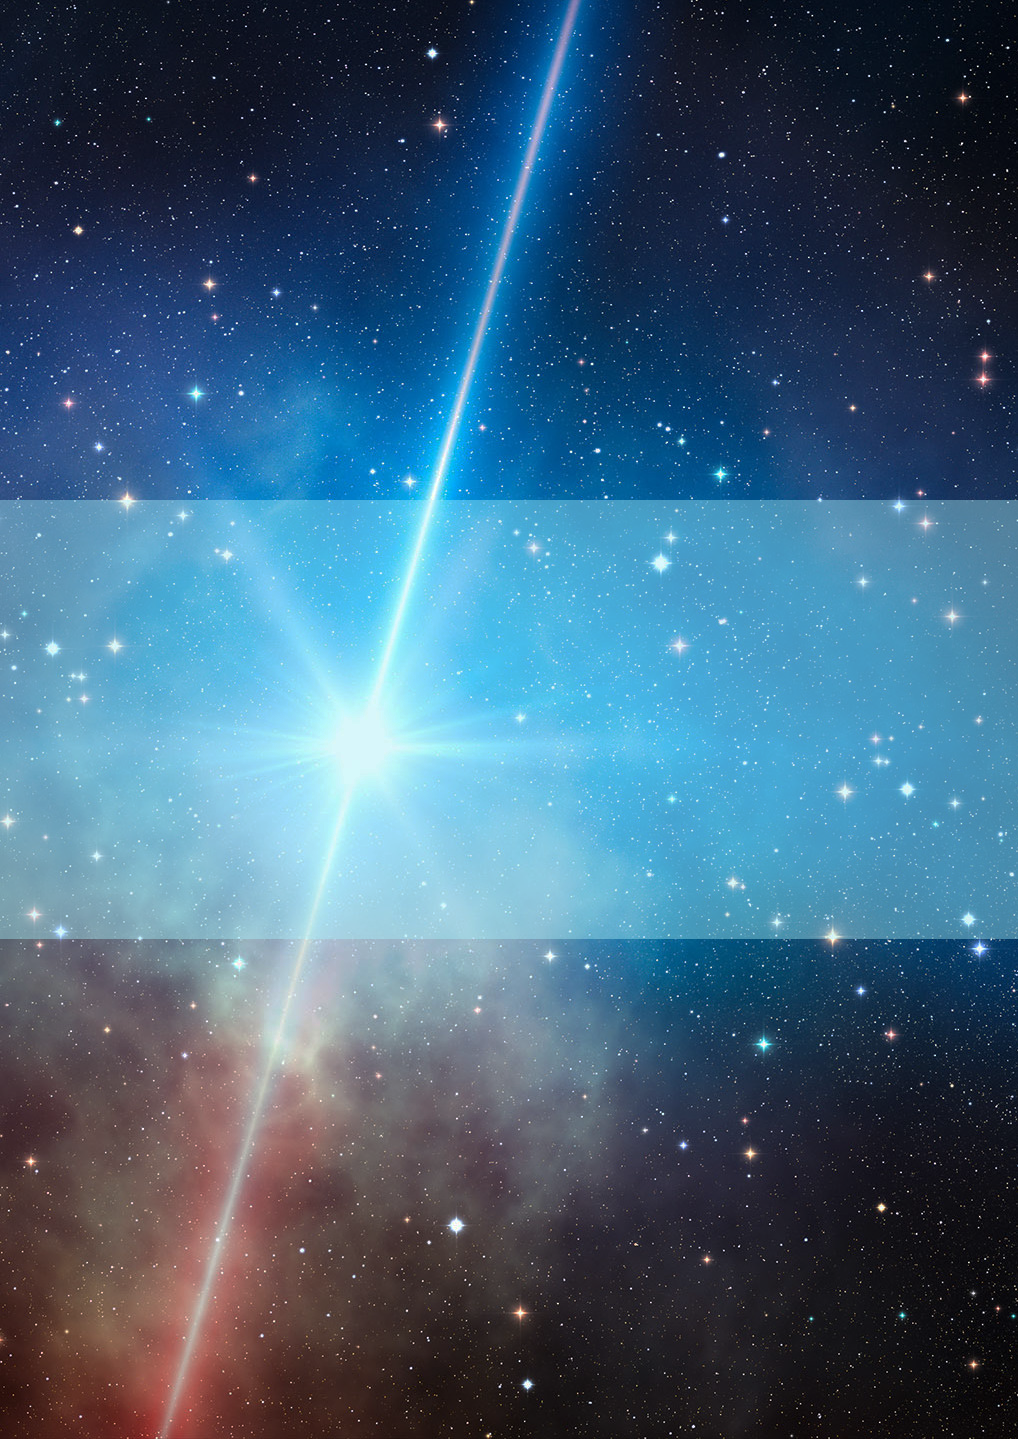
\includegraphics[height=\paperheight, width=\paperwidth]{Pictures/cover.png}}
        \end{center}
	\vspace*{25em}
	{\centering
	\makeatletter
		\@title\\[0.5em]
		{\normalfont\LARGE\printauthorlist}
	\makeatother
	}
	\endgroup

\end{titlepage}

%----------------------------------------------------------------------------------------
%	COPYRIGHT/ALT TITLE PAGE
%----------------------------------------------------------------------------------------

\begin{titlepage}
	\thispagestyle{empty}
	\date{\protect\raggedright
		\vfill
		\noindent Copyright \copyright\ 2023 Krittika IITB\\ %Copyright notice
		\noindent \textsc{Published by Krittika: The Astronomy Club of IIT Bombay}\\ % Publisher	
		\noindent \href{https://github.com/krittikaiitb}{\textsc{github.com/krittikaiitb}} \\ % URL
	First Release, July 2023 % Printing/edition date
}
	\maketitle
\end{titlepage}

%----------------------------------------------------------------------------------------
%	ABSTRACT
%----------------------------------------------------------------------------------------

\newpage
\pagestyle{empty}
\begin{center}
{\huge \textmd{Abstract}}\\
\end{center}
\vspace{5em}


%----------------------------------------------------------------------------------------
%	TABLE OF CONTENTS
%----------------------------------------------------------------------------------------

% \usechapterimagefalse % If you don't want to include a chapter image, use this to toggle images off - it can be enabled later with \usechapterimagetrue

\chapterimage{index} % Table of contents heading image

\pagestyle{empty} % Disable headers and footers for the following pages
%\setcounter{tocdepth}{0}
\tableofcontents % Print the table of contents itself

\pagestyle{fancy} % Enable headers and footers again

%----------------------------------------------------------------------------------------
%	CHAPTER 1
%----------------------------------------------------------------------------------------

\chapterimage{astrosat} % Chapter heading image

\chapter{Introduction}
\section{Gamma Ray Bursts}
\subsection{What are Gamma Ray Bursts?}
Gamma-ray bursts (GRBs) are massively large explosions caused when a star dies resulting in a supernova, when two \href{https://en.wikipedia.org/wiki/Neutron_star}{neutron stars} collide, or when a neutron star collides with a \href{https://en.wikipedia.org/wiki/Black_hole}{black hole}, releasing a large amount of energy.  

\begin{figure}[H]
\centering
    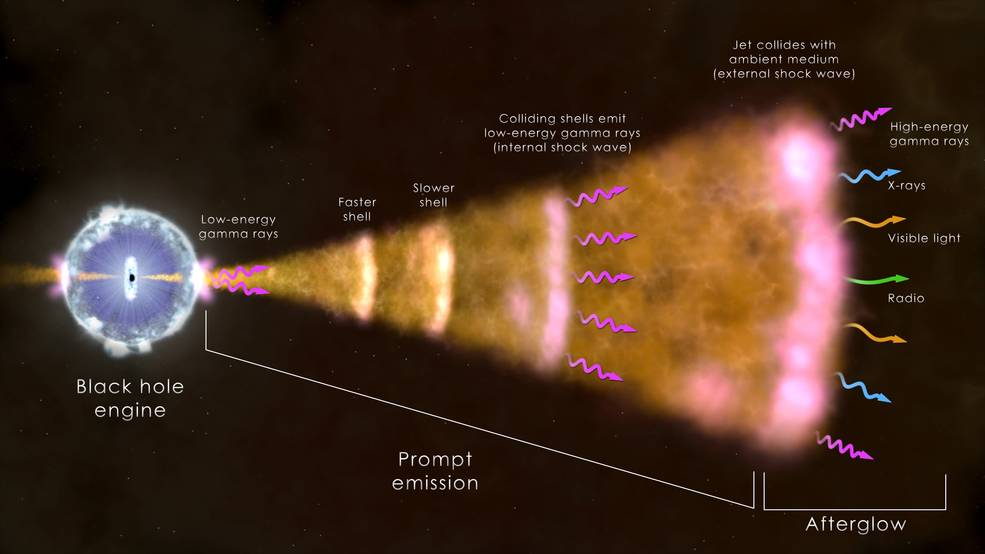
\includegraphics[width=0.7\textwidth]{Pictures/grb_shell_final_0.jpg}
    \caption{Emissions of a GRB (Source: \href{https://www.nasa.gov/feature/goddard/2023/nasa-missions-study-what-may-be-a-1-in-10000-year-Gamma-ray-burst}{NASA's Goddard Space Flight Center})}
\end{figure}

This illustration shows the ingredients of a long Gamma-ray burst, the most common type. The core of a massive star (left) has collapsed, forming a black hole that sends a jet of particles moving through the collapsing star and out into space at nearly the speed of light. Radiation across the spectrum arises from hot ionized gas (plasma) in the vicinity of the newborn black hole, collisions among shells of fast-moving gas within the jet (internal shock waves), and from the leading edge of the jet as it sweeps up and interacts with its surroundings (external shock). The presence of a prompt emission and a much longer afterglow (in multiple wavelengths) is a common feature of GRBs.

\subsection{Classification of GRBs}
GRBs are classified into 3 main classes, short, long and ultra-long, according to the duration for which they are detected.

\begin{wrapfigure}[15]{r}{0.4\textwidth}
    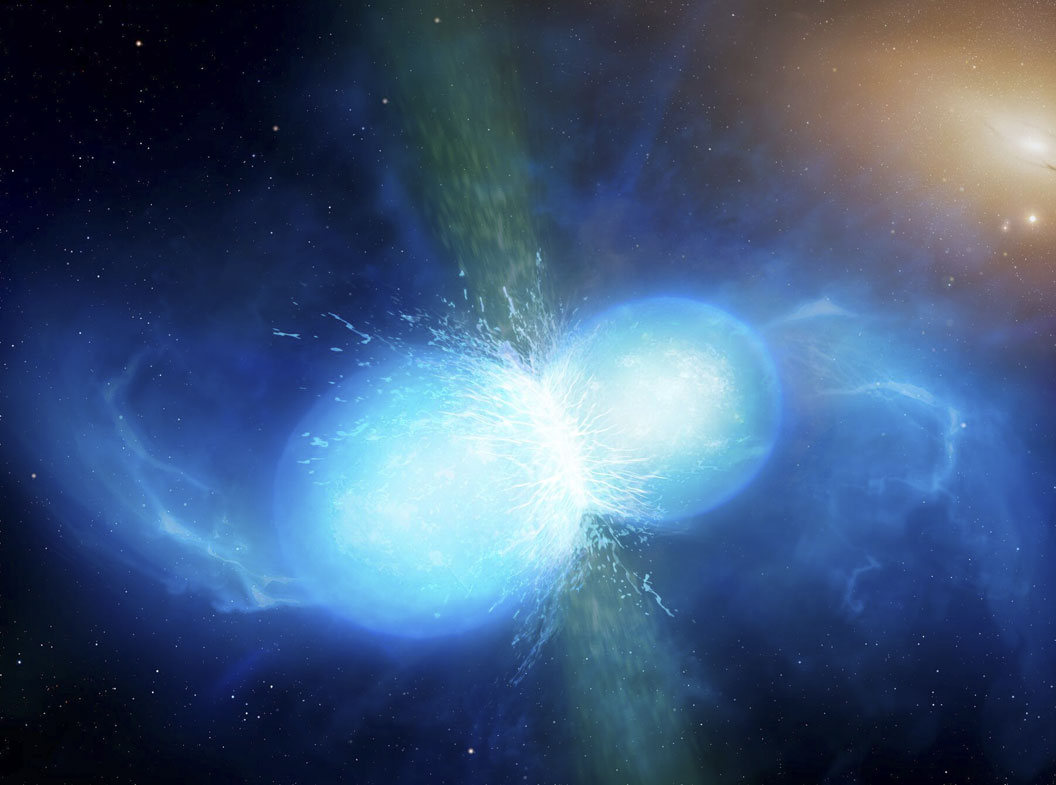
\includegraphics[width=0.4\textwidth]{Pictures/neutronstars.jpg}
    \caption{Artist depiction of a GRB created by two merging neutron stars (Source: \href{http://www.markgarlick.com/index.html}{Mark A. Garlick})}
\end{wrapfigure}

\textbf{Short GRBs} are events with a duration of less than 2 seconds, and the Gamma rays from short bursts lean toward the high-energy end of the spectrum, while long GRBs emit lower-energy Gamma rays. They are thought to be caused by the merger of two neutron stars or a neutron star and a black hole and account for about 30\% of detected GRBs.


\textbf{Long GRBs} are events with a duration of more than 2 seconds. Although the Gamma rays emitted are of lower energy than short GRBs, the total energy output of long GRBs is generally higher owing to their longer duration. They are thought to be caused by the core collapse of rapidly rotating massive stars 

\textbf{Ultra-Long GRBs} are events that last more than 10,000 seconds. They have been proposed to be caused by the collapse of a \href{https://en.wikipedia.org/wiki/Blue_supergiant}{Blue Supergiant} star, a \href{https://en.wikipedia.org/wiki/Tidal_disruption_event}{tidal disruption event} or a newborn \href{https://en.wikipedia.org/wiki/Magnetar}{magnetar}

\section{Astrosat and CZTI}
\subsection{Astrosat - India's first multiwavelength space telescope}
AstroSat is the first dedicated Indian astronomy mission aimed at studying celestial sources in X-ray, optical and UV spectral bands simultaneously. The payloads cover the energy bands of Ultraviolet (Near and Far), limited optical and X-ray regime (0.3 keV to 100keV). One of the unique features of AstroSat mission is that it enables the simultaneous multi-wavelength observations of various astronomical objects with a single satellite.

AstroSat with a lift-off mass of 1515 kg was launched on September 28, 2015 into a 650 km orbit inclined at an angle of 6 deg to the equator by PSLV-C30 from Satish Dhawan Space Centre, Sriharikota. The minimum useful life of the AstroSat mission is expected to be 5 years.


\begin{wrapfigure}{l}{0.4\textwidth}
    \centering
    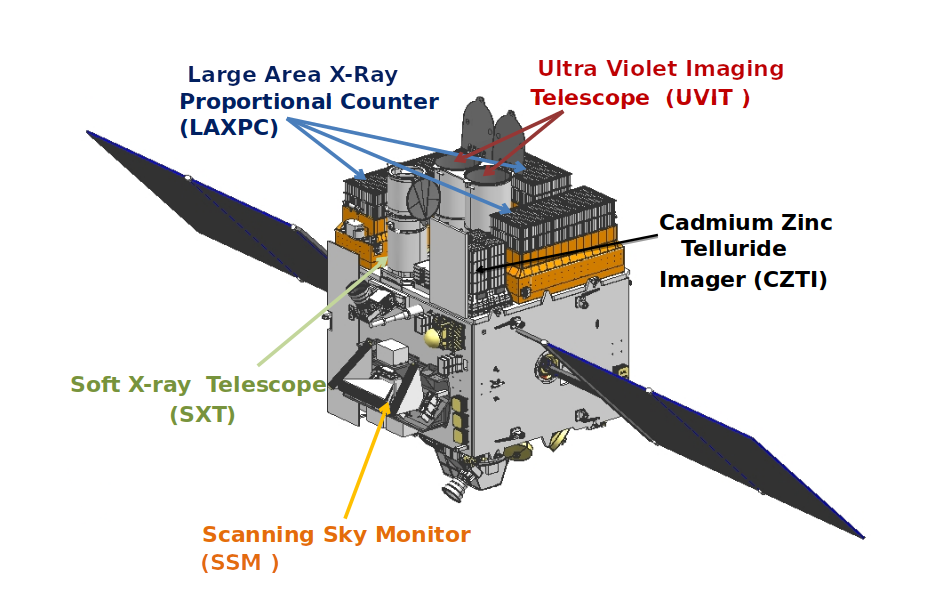
\includegraphics[scale=0.8]{Pictures/astrosat_wireframe.png}
    \caption{Various Payloads on Astrosat (Source: \href{https://webapps.issdc.gov.in/astro_archive/archive/astrosat_images/astrosat_wireframe.png}{ISSDC})}
\end{wrapfigure}

The spacecraft control centre at Mission Operations Complex (MOX) of ISRO Telemetry, Tracking and Command Network (ISTRAC), Bengaluru manages the satellite during its entire mission life. The science data gathered by five payloads of AstroSat are telemetered to the ground station at MOX. The data is then processed, archived and distributed by Indian Space Science Data Centre (ISSDC) located at Bylalu, near Bengaluru.

\clearpage



\subsection{Cadmium-Zinc-Telluride Imager (CZTI)}


\begin{wrapfigure}[18]{r}{0.4\textwidth}
    \centering
    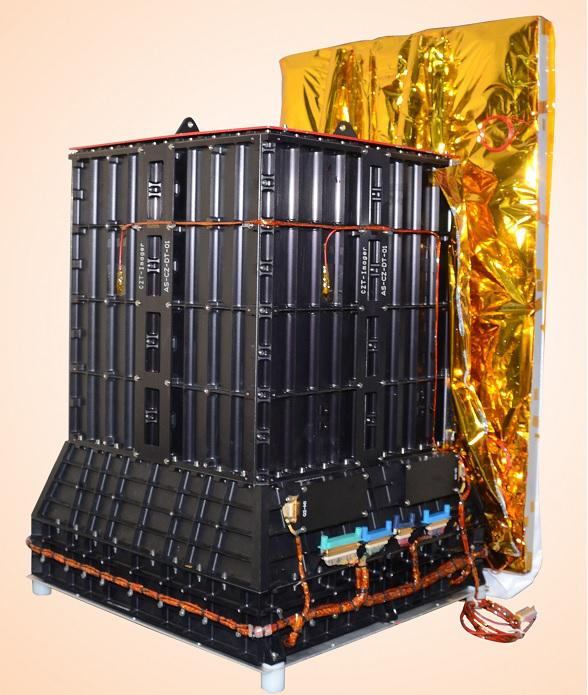
\includegraphics[scale=1]{Pictures/czti.jpg}
\caption{CZTI (Source: \href{http://astrosat.iucaa.in/czti/?q=home}{IUCAA})}
\end{wrapfigure}

It is a hard X-ray imaging instrument covering the energy band from 10 to 100 keV, has a detector area of 976 cm$^2$ constructed using CZT modules, and uses a Coded Aperture Mask (CAM) for imaging.
The CZTI carries a Cesium Iodide (Tl) based scintillator detector for Veto measurements. This is located just under the CZT detector modules. Further, there is a gap of about 8 cm between the base of the collimator slats and the detector plane, in order to accommodate a radioactive calibration source module in each quadrant. This source shines alpha-tagged 60 keV photons on the CZT detector in order to help calibrate the energy response.

Veto Detector - a detector (CsI) covers the large area of 256 cm2 and the light collection is done using two photomultipliers (PMT), viewed from sides. On registering an event, a signal from the detector is sent to a pre-amplifier. This signal is processed and sent to the FEB for further analysis. After amplification of the signal from pre-amplifier, the signal is sent to a comparator via stretcher along with LLD level signal. If LLD is triggered the pulse is digitized to an 8-bit output by ADC through control circuit. This output is used to differentiate Compton scattered events and hence the background in main detector can be reduced.

\begin{wrapfigure}[16]{l}{0.4\textwidth}
    \centering
    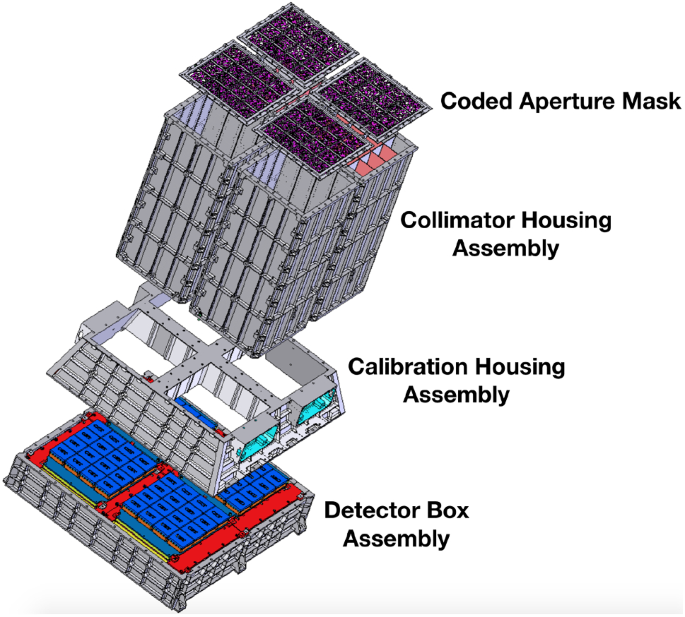
\includegraphics[scale=0.25]{Pictures/cztiassembly.png}
    \caption{CZTI Assembly (Source: \href{https://arxiv.org/pdf/2108.06746.pdf}{Image Calibration Paper})}
\end{wrapfigure}

The full CZTI detector is illuminated
only by the on-axis source. Off-axis sources illuminate
only a part of the detector depending on the position of
the source, this is called “partial coding”. The coded
mask for CZTI is designed with seven patterns based
on 255-element pseudo-noise Hadamard set Uniformly
Redundant Arrays (URA).  Each
pattern has 16×16 mask elements and used as a mask for an individual detector module. A random arrangement of these patterns into a 4 × 4 array results in the mask pattern for the first quadrant (quadrant A). The coded masks for the other quadrants (B, C, and D) were
obtained by rotating the mask pattern of quadrant A by
90°, 180° and 270° respectively.

A passive collimator wall of height 400 mm separates any two adjacent modules, restricting the view
of each detector module to the coded mask directly
above it. The collimator thus restricts the Field of View
(FOV) of CZTI to 4.6° × 4.6° FWHM at energies below
100 keV. For energies above 100 keV, the collimator
walls and the coded mask become progressively transparent, and allows the detection of Gamma-Ray Bursts
from all over the sky

\clearpage


\subsection{Coded Aperture Mask Imaging}

%\vspace{-1.1cm}

\begin{wrapfigure}[17]{r}{0.5\textwidth}
    \centering
    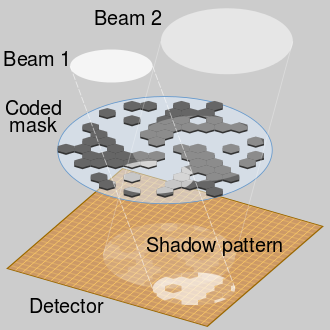
\includegraphics[scale=0.53]{Pictures/cam_working.png}
\caption{Working of a CAM (Source: \href{https://en.wikipedia.org/wiki/Coded_aperture}{Wikipedia})}
\end{wrapfigure}


Coded apertures or coded-aperture masks are grids, gratings, or other patterns of materials opaque to various wavelengths of electromagnetic radiation. The wavelengths are usually high-energy radiation such as X-rays and Gamma rays. By blocking radiation in a known pattern, a coded "shadow" is cast upon a plane. The properties of the original radiation sources can then be mathematically reconstructed from this shadow. Coded apertures are used in X- and Gamma ray imaging systems, because these high-energy rays cannot be focused with lenses or mirrors that work for visible light. 

\begin{figure}[H]
    \centering
    
\includegraphics[scale=0.69]{Pictures/CAM-czti.png}
    \caption{CZTI coded aperture mask for all four quadrants designed using 255 element pseudo-noise Hadamard
    set Uniformly Redundant Arrays. One extra closed element is added to each URA to obtain a square pattern. Here
    black areas represent closed mask elements and white areas represent open ones. (Source: \href{https://arxiv.org/pdf/2108.06746.pdf}{Image Calibration Paper})}
\end{figure}

\clearpage

\section{CZT Pipeline}

\subsection{How It Works}
The data received from the CZTI payload passes through a series of steps in a processing
pipeline. Three major data levels have been designated for long-term storage. These are:

\noindent\textbf{Level 0}

This is the raw data received from satellite telemetry, which is segregated by instrument,
along with auxiliary data. This data is archived internally and not distributed for public
use.

\noindent\textbf{Level 1}

This is reorganized raw data, written in FITS format for Astronomical use. All auxiliary
information necessary for further processing of this data are collated at this level and
packed along with the respective science data. This data is released via Astrosat data
archive, at first to the Principal Investigator (PI) of the corresponding observing proposal
and, after a specified initial lock in period, to anyone interested in the data.

\noindent\textbf{Level 2}

This data contains standard science products derived from Level 1 data. Level 2 data is
also in FITS format and is available for science use, with the same lock-in criteria and
release mechanism as the Level 1 data.

\begin{figure}[H]
    \centering
    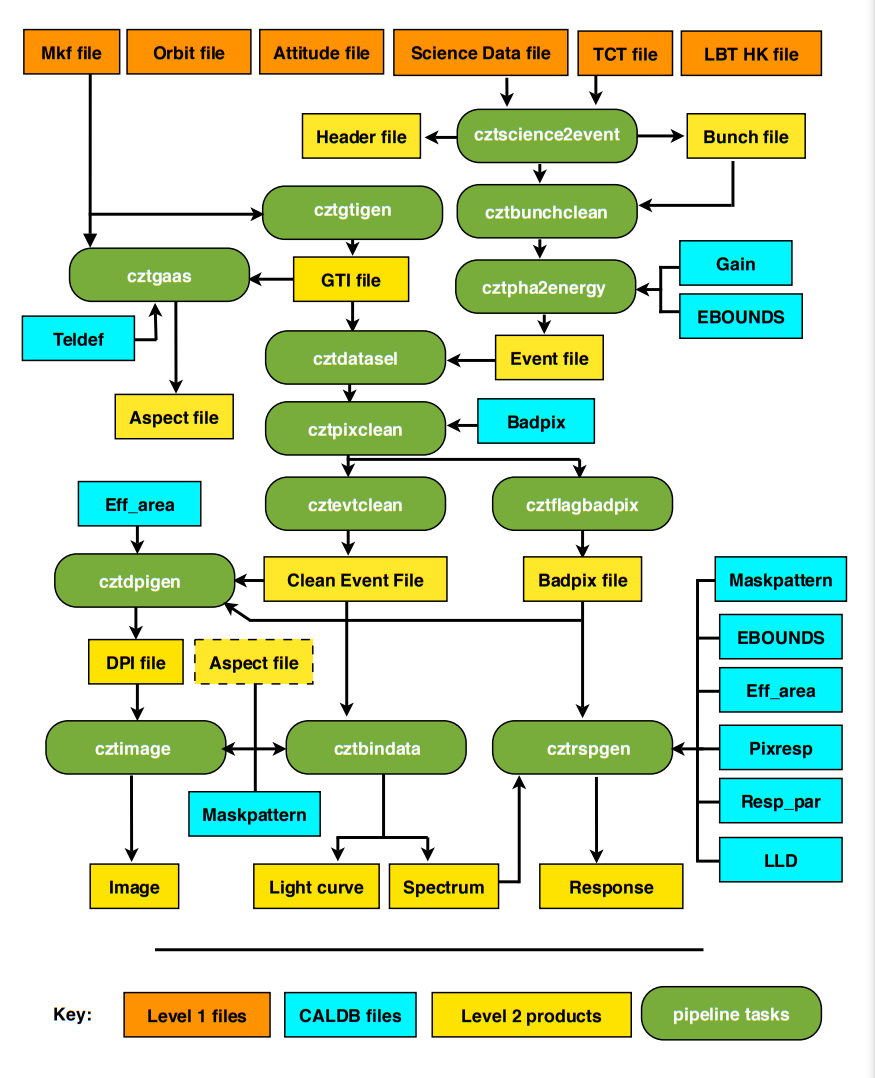
\includegraphics[scale=0.55]{Pictures/cztpipeline.png}
    \caption{Pipeline Work Flow (Source: \href{http://astrosat-ssc.iucaa.in/uploads/czti/CZTI_level2_software_userguide_V2.1.pdf}{CZT Software Userguide})}
\end{figure}

\subsection{Work Flow}

Data reduction for CZTI is performed in three stages. Each of these stages involves
execution of several tasks of the pipeline.

\begin{itemize}
    \item Stage 1: Generation of event file and calibration. In this stage event file is generated
    \item Stage 2: Selection of data and cleaning. In this stage events are selected based on Good Time Interval and noisy pixel events are removed from the data.
    \item Stage 3: Generation of science products. In this last stage,DPI, image, spectrum, light curve and response matrix are generated.
\end{itemize}

The pipeline tasks can either be executed individually or by using the cztpipeline
module which allows the user to run required stages of the pipeline tasks.


\subsection{Pipeline Installation}

I found Ubuntu 20.04 LTS to work best with the pipeline on WSL2. Other distros (including other versions of Ubuntu) gave various compilation errors.

To start off, update the system by running 
\begin{lstlisting}{language=bash}
    $ sudo apt update && sudo apt upgrade
\end{lstlisting}

After this, we must install some packages that are essential to ensuring the pipeline installs smoothly. Install them by running 
\begin{lstlisting}{language=bash}
    $ sudo apt install gcc g++ gfortran perl make
\end{lstlisting}


Now download the pipeline from \href{http://astrosat-ssc.iucaa.in/uploads/czti/czti_pipeline_20180308_V2.1.tar}{here} and the CALDB from \href{http://astrosat-ssc.iucaa.in/uploads/czti/caldb_goodfiles_as1_czti_20180308_V1.1.tar.gz}{here}. 

Untar these files, ideally in your home directory by running the following:
\begin{lstlisting}{language=bash}
    $ tar -xvf czti_pipeline_20180308_V2.1.tar
    $ tar -xvf caldb_goodfiles_as1_czti_20180308_V1.1.tar.gz
\end{lstlisting}


Now add the following to your \lstinline[language=bash]{.bashrc} file (by running \lstinline[language=bash]{$ sudo nano ~/.bashrc})
\begin{lstlisting}{language=bash}
    export as1czt=~/czti_pipeline/CZTI/czti/
    export PFILES="$PFILES:$as1czt/paramfiles"
    export PATH=$as1czt/bin:$as1czt/scripts:$PATH
    export GLOG_log_dir=$as1czt/log
    export CZTI_templates=$as1czt/templates
    export PERL5LIB="$as1czt/lib/":$PERL5LIB
    export LD_LIBRARY_PATH=$LD_LIBRARY_PATH:$as1czt/lib
    export PYTHONPATH="$PYTHONPATH:$as1czt/scripts"
    export CXXFLAGS="-fpermissive"
    ulimit -s 65532
    export CALDB=~/
\end{lstlisting}


Finally execute the following commands

\begin{lstlisting}{language=bash}
    $ source ~/.bashrc
    $ cd $as1czt
    $ cd ../
    $ ./InstallLibs
    $ cd $as1czt
    $ make
    $ cd scripts
    $ chmod +x cztpipeline
\end{lstlisting}

\subsection{Automation of the Pipeline}
% In a joint effort with \href{}{Shreyas N.B.} we have automated the pipeline using python. The code uses the subprocess module to run the pipeline commands in the terminal, along with the \lstinline[language=python]{tkinter} module to create a GUI for the user to interact with. The code can be found \href{}{here}


%----------------------------------------------------------------------------------------
%	CHAPTER 2
%----------------------------------------------------------------------------------------
\chapterimage{Pictures/BOAT.png}
\chapter{Playing With Data}

\section{Introduction}

\subsection{FITS Files}

FITS (Flexible Image Transport System) is a standard format for storing astronomical data. FITS is much more than an image format (such as JPG or GIF) and is primarily designed to store scientific data sets consisting of multi-dimensional arrays (1-D spectra, 2-D images or 3-D data cubes) and 2-dimensional tables containing rows and columns of information.

\noindent\textbf{Headers}

The FITS header is a block of text at the beginning of the file that contains information about the data contained within the file. The header is arranged in a series of keyword-value pairs, known as header cards, that each consist of a keyword, a value, and an optional comment. The keyword tells the type of information that the header card contains, the value is the actual value of the information, and the comment describes the information or how it was derived. The header is terminated by the keyword END.

\noindent\textbf{Data}

The data in a FITS file is stored in a series of N-dimensional arrays, where N is any number between 0 (empty) and 999. The data arrays are preceded by a series of header keywords that describe the size (NAXIS), location (NAXISn), data type (BITPIX), and other characteristics of the data arrays. The data arrays are stored in the file in the same order that they are listed in the header.

\subsection{Accessing Files via Astropy}

Astropy is a community Python library for Astronomy. It contains among other things:

\begin{itemize}
    \item A powerful N-dimensional array object
    \item Sophisticated (broadcasting) functions
    \item Tools for integrating Fortran code
    \item Useful linear algebra, Fourier transform, and random number capabilities
\end{itemize}

Opening a FITS file is as simple as:

\begin{lstlisting}[language=Python]
    from astropy.io import fits
    hdul = fits.open('file.fits')
    hdul.info()
\end{lstlisting}

This will print out the information about the file, including the number of HDUs in the file and the name and dimensions of each extension.

To obtain the data and header from the file, we can use:

\begin{lstlisting}[language=Python]
    data = hdul[0].data
    header = hdul[0].header
\end{lstlisting}


\subsection{Creating the Light Curve Files}

The light curve files are created by running the \lstinline[language=bash]{cztbindata} command in the terminal. The command takes in the following input files along with time bin size and produces the .lc and .pha (spectrum) file:

\begin{itemize}
    \item \lstinline[language=bash]{inevtfile} - The input evt file
    \item \lstinline[language=bash]{mkffile} - The input mkf file
    \item \lstinline[language=bash]{badpixfile} - The input badpix file
    \item \lstinline[language=bash]{livetimefile} - The input livetime file
\end{itemize}

Finally the .lc file can be opened using \lstinline[language=Python]{astropy.io.fits} and the required columns can be plotted. In our case we will be plotting the \lstinline[language=Python]{COUNTS} column against the \lstinline[language=Python]{TIME} column.

Here is a sample light curve file plotted for the duration of the GRB190928A:

\begin{figure}[H]
    \centering
    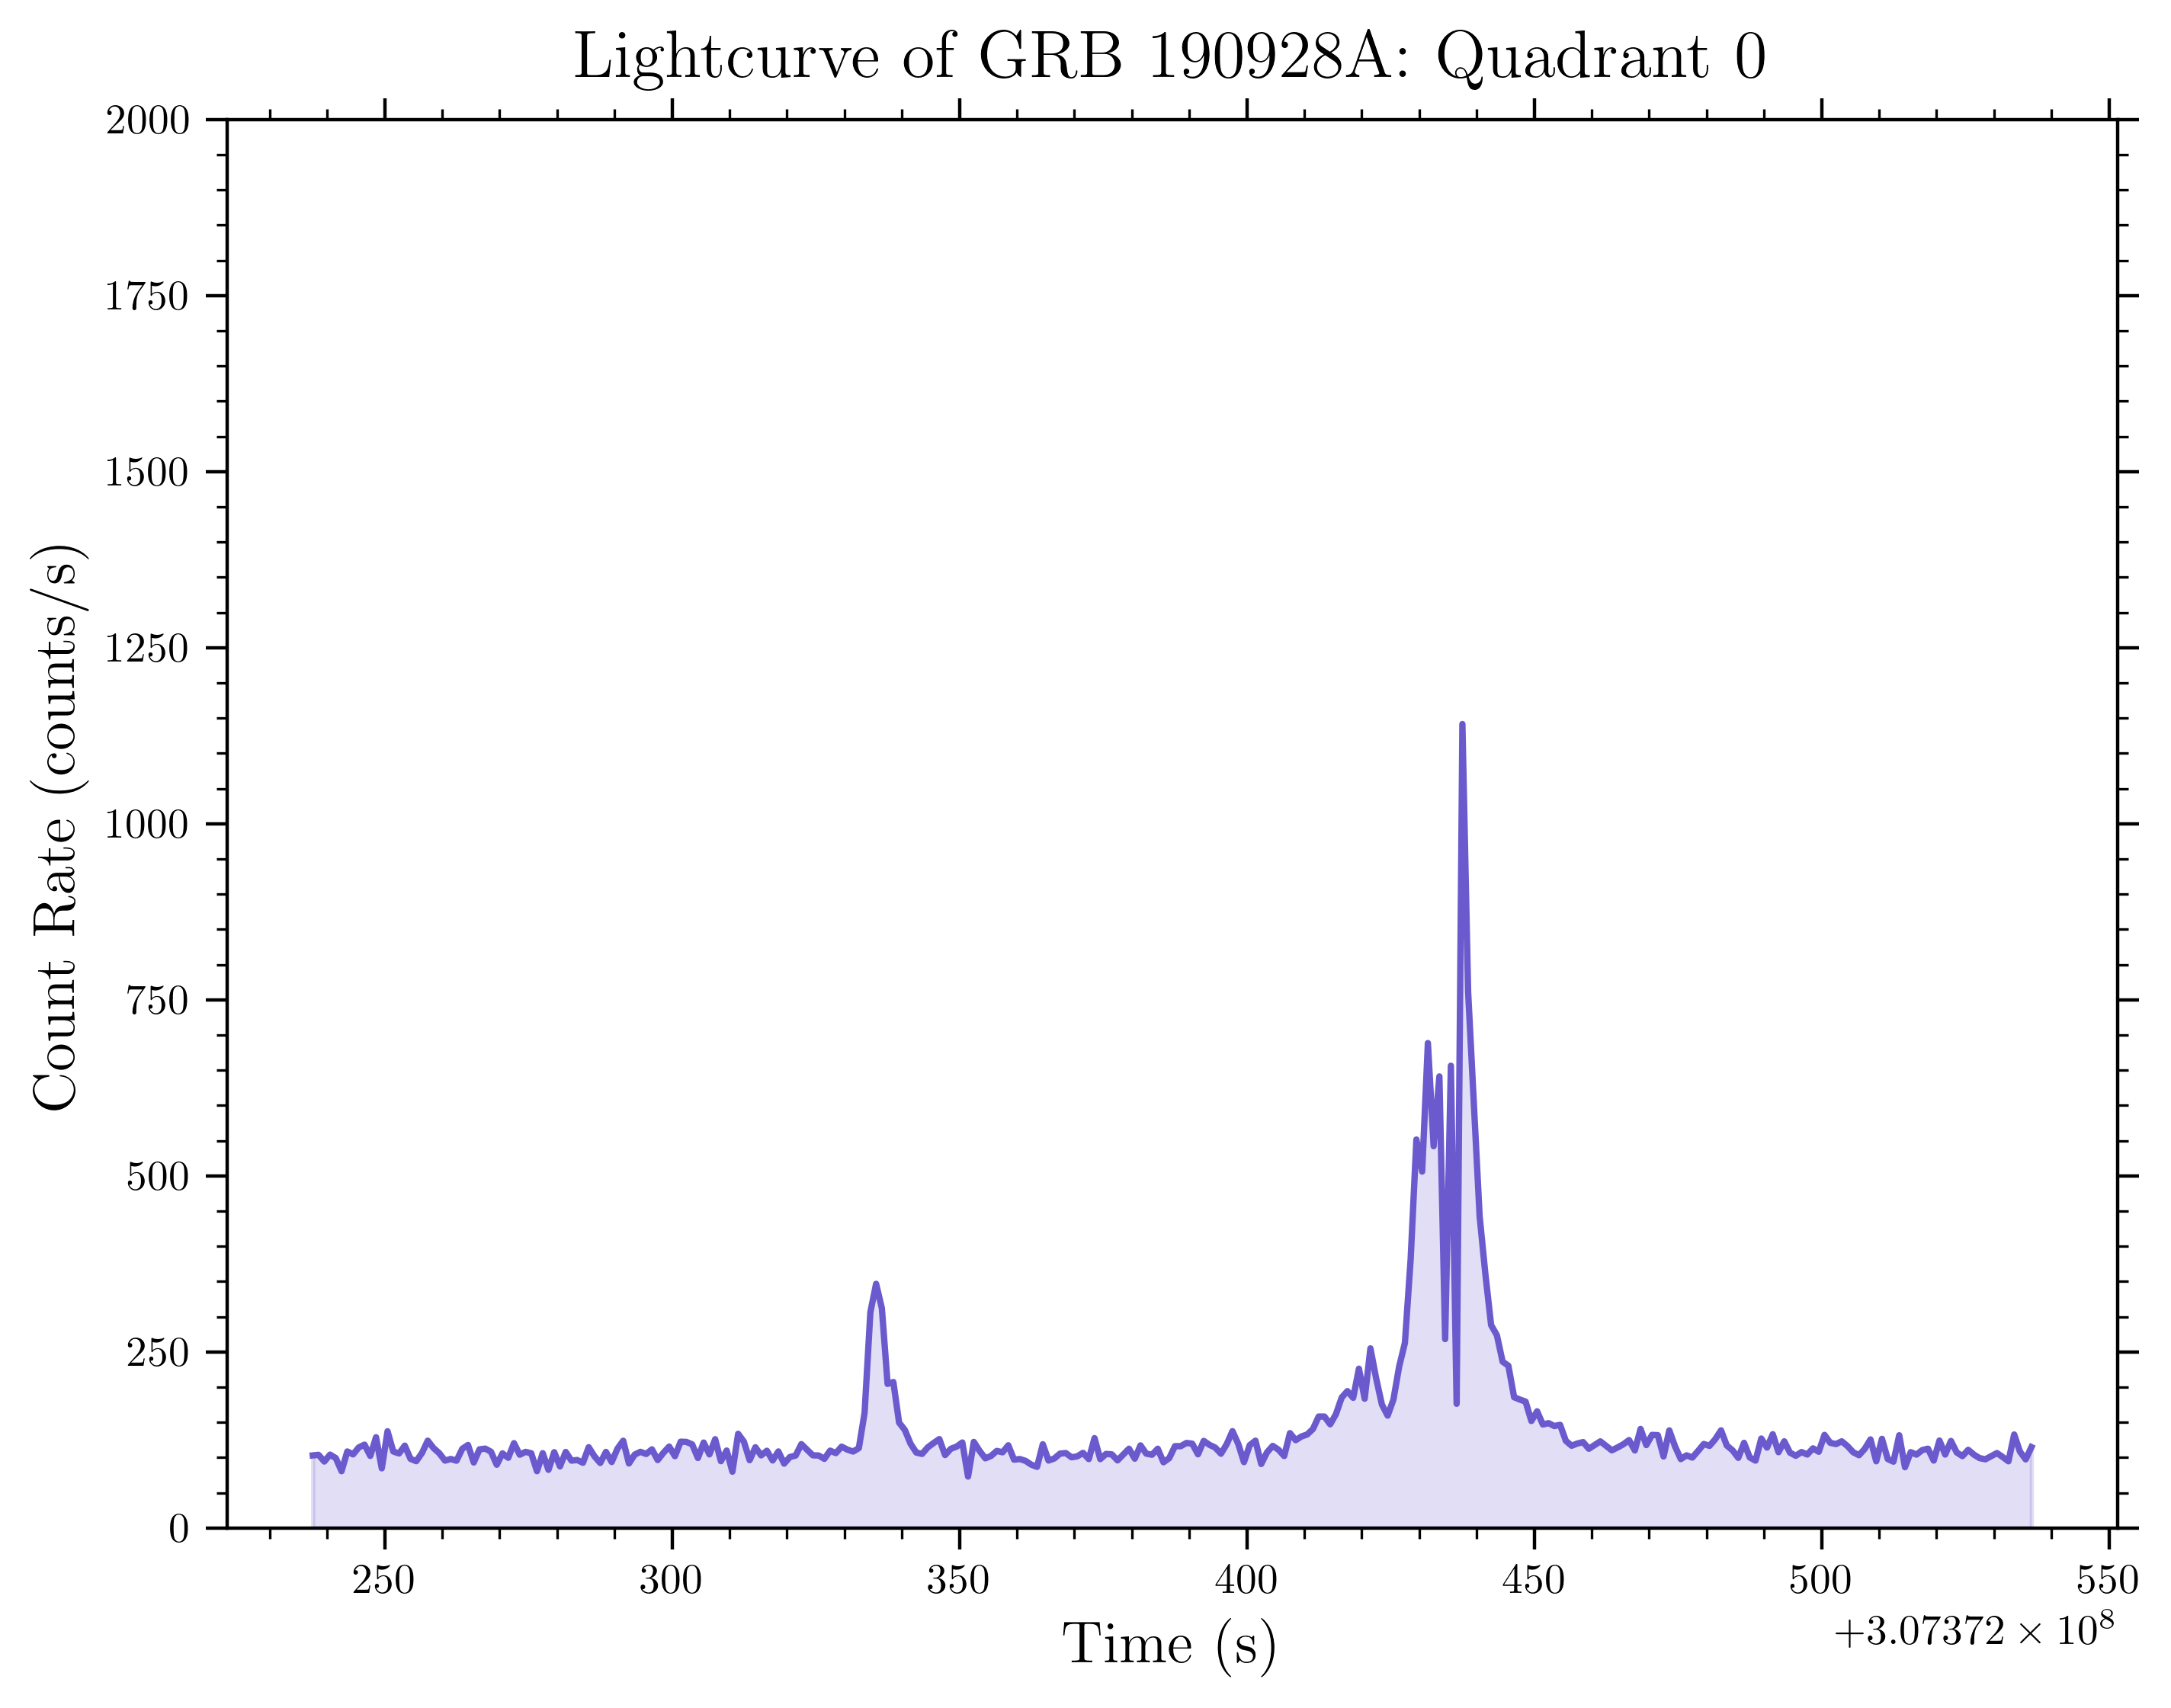
\includegraphics[scale=0.65]{Pictures/sample_lc.png}
    \caption{Light Curve for GRB190928A}
\end{figure}

\subsection{Creating the Spectrum Files}

The process used in creating the light curve will automatically produce a .pha file which contains the spectrum of the GRB. We can plot the spectrum using \lstinline[language=Python]{astropy.io.fits} and \lstinline[language=Python]{matplotlib.pyplot}.

\begin{figure}[H]
    \centering
    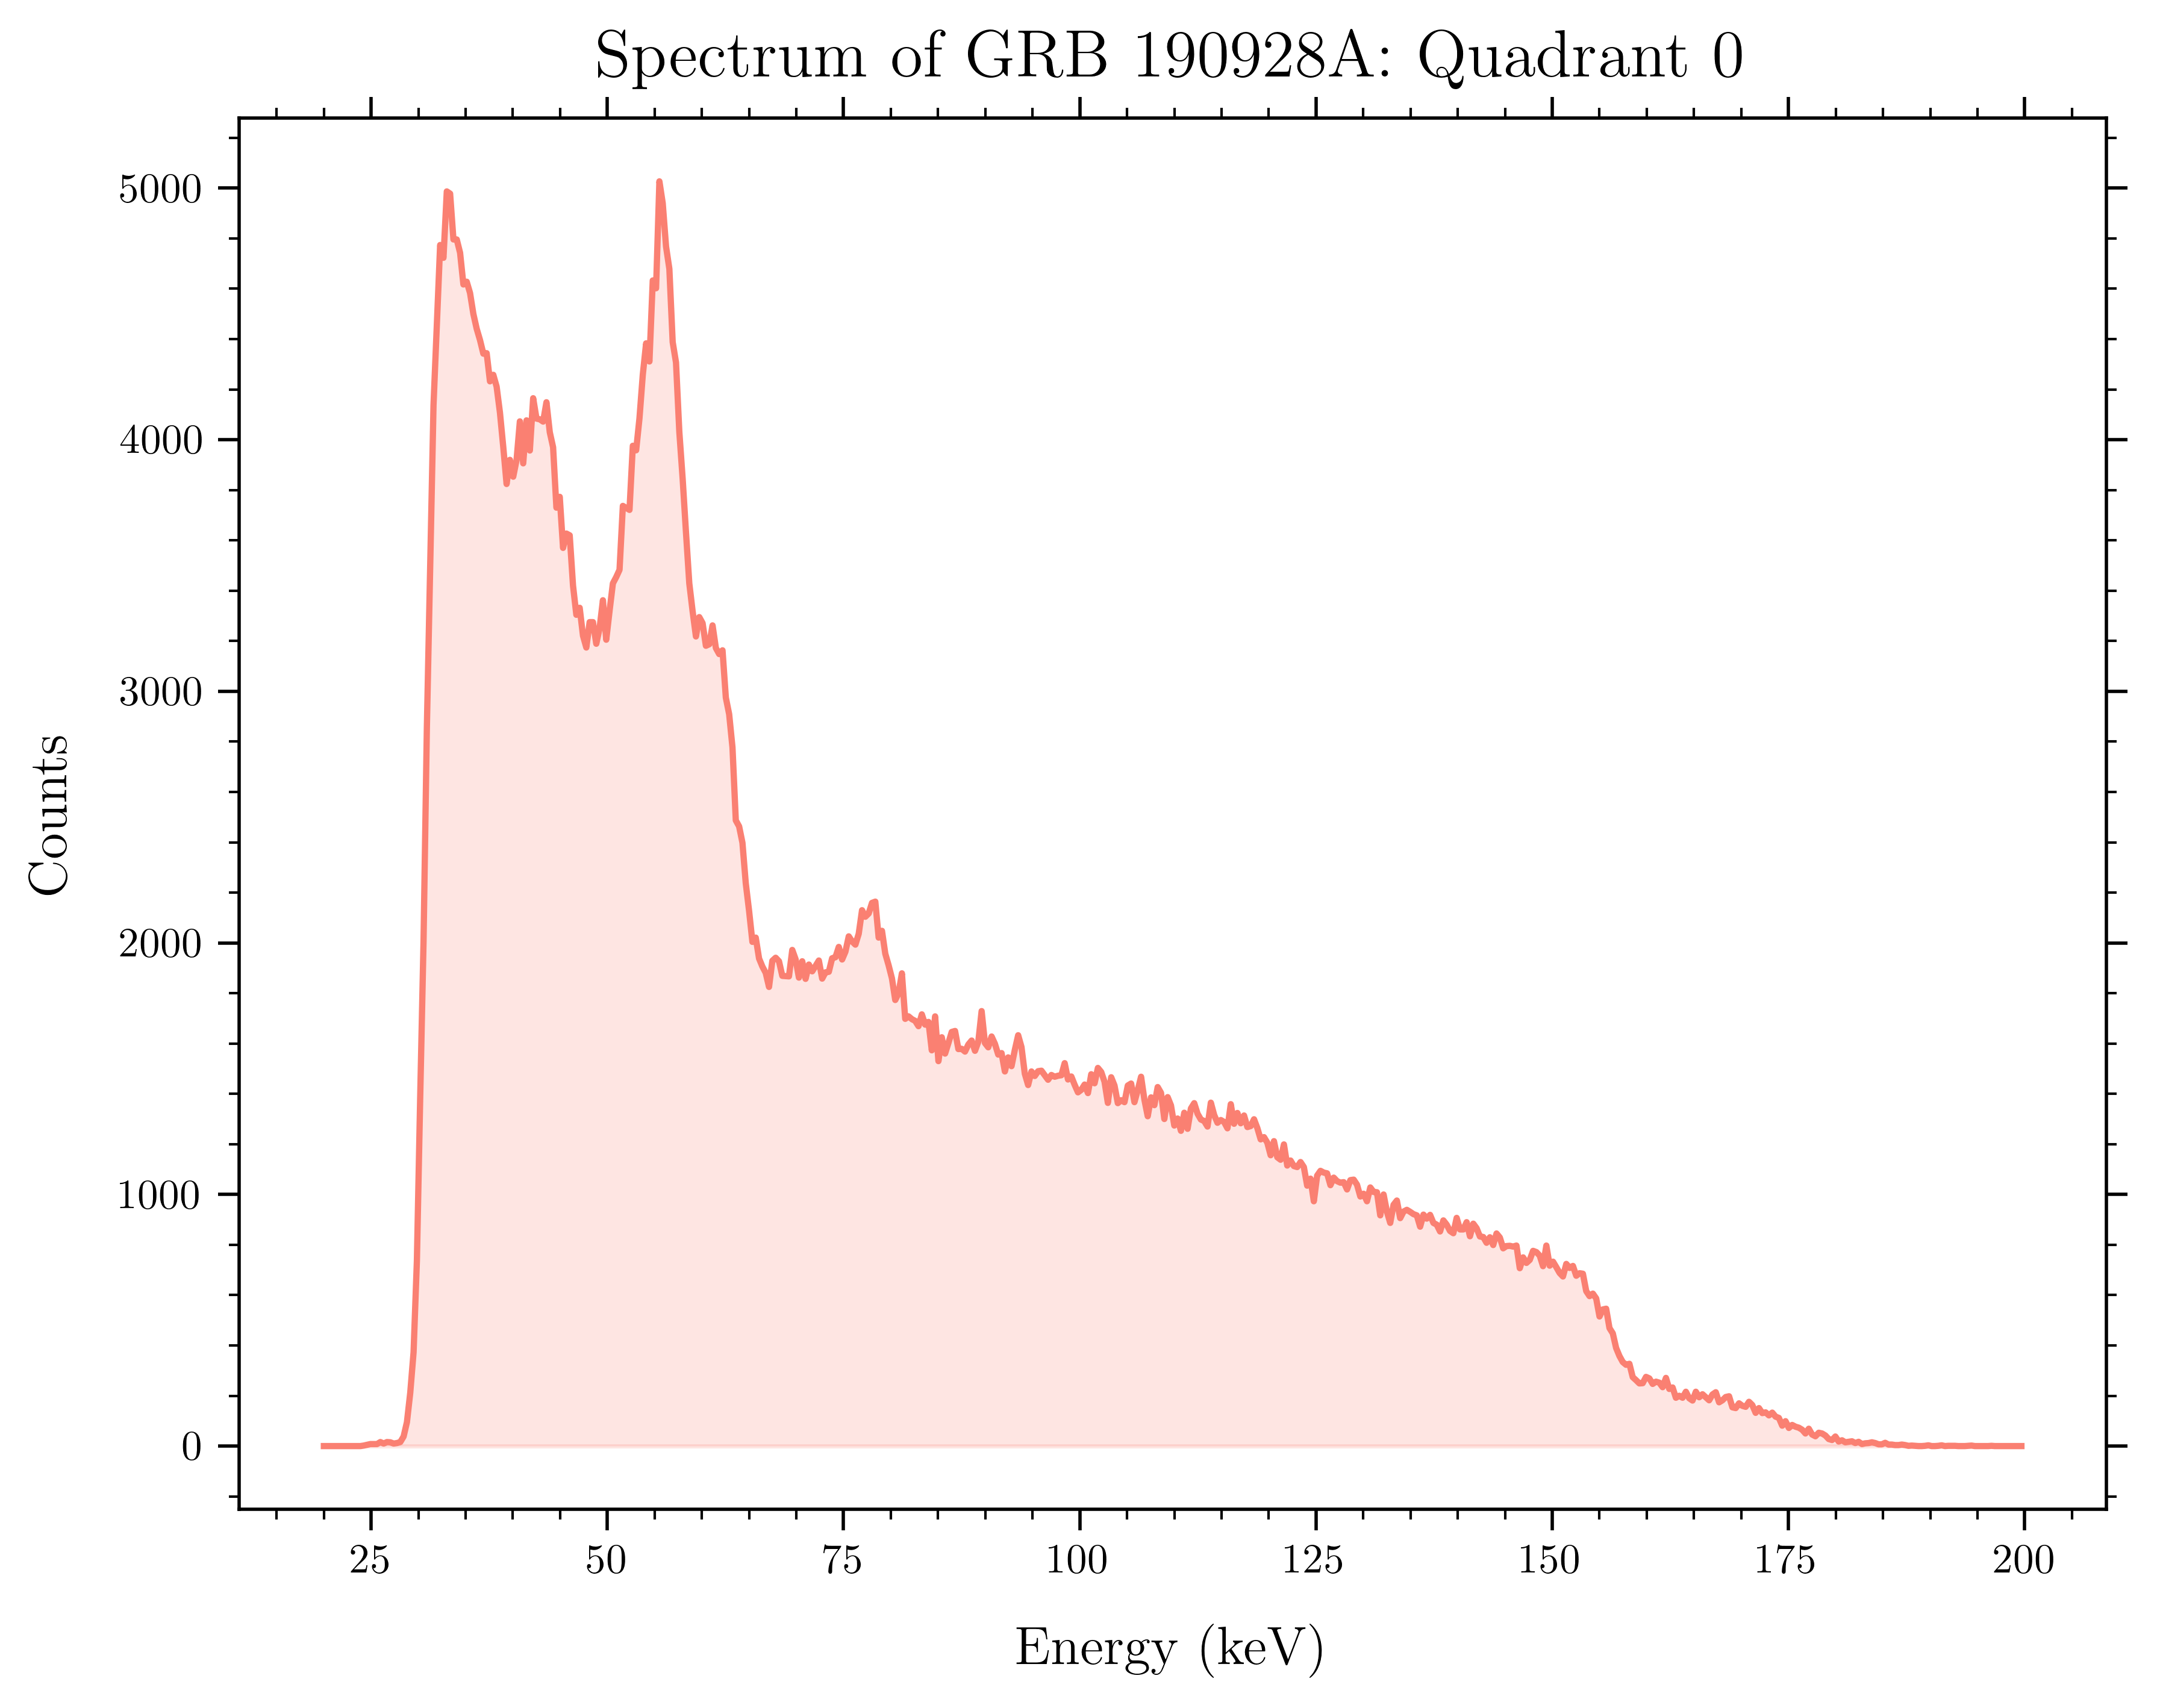
\includegraphics[scale=0.55]{Pictures/spectrum.png}
    \caption{Spectrum for GRB190928A}
\end{figure}

\subsection{Some Anomalies in the Data}

The above light curve was plotted around the time of the GRB, but if we plot the full light curve, we can see some anomalies in the data where the counts suddenly fall to zero.
\begin{figure}[H]
    \centering
    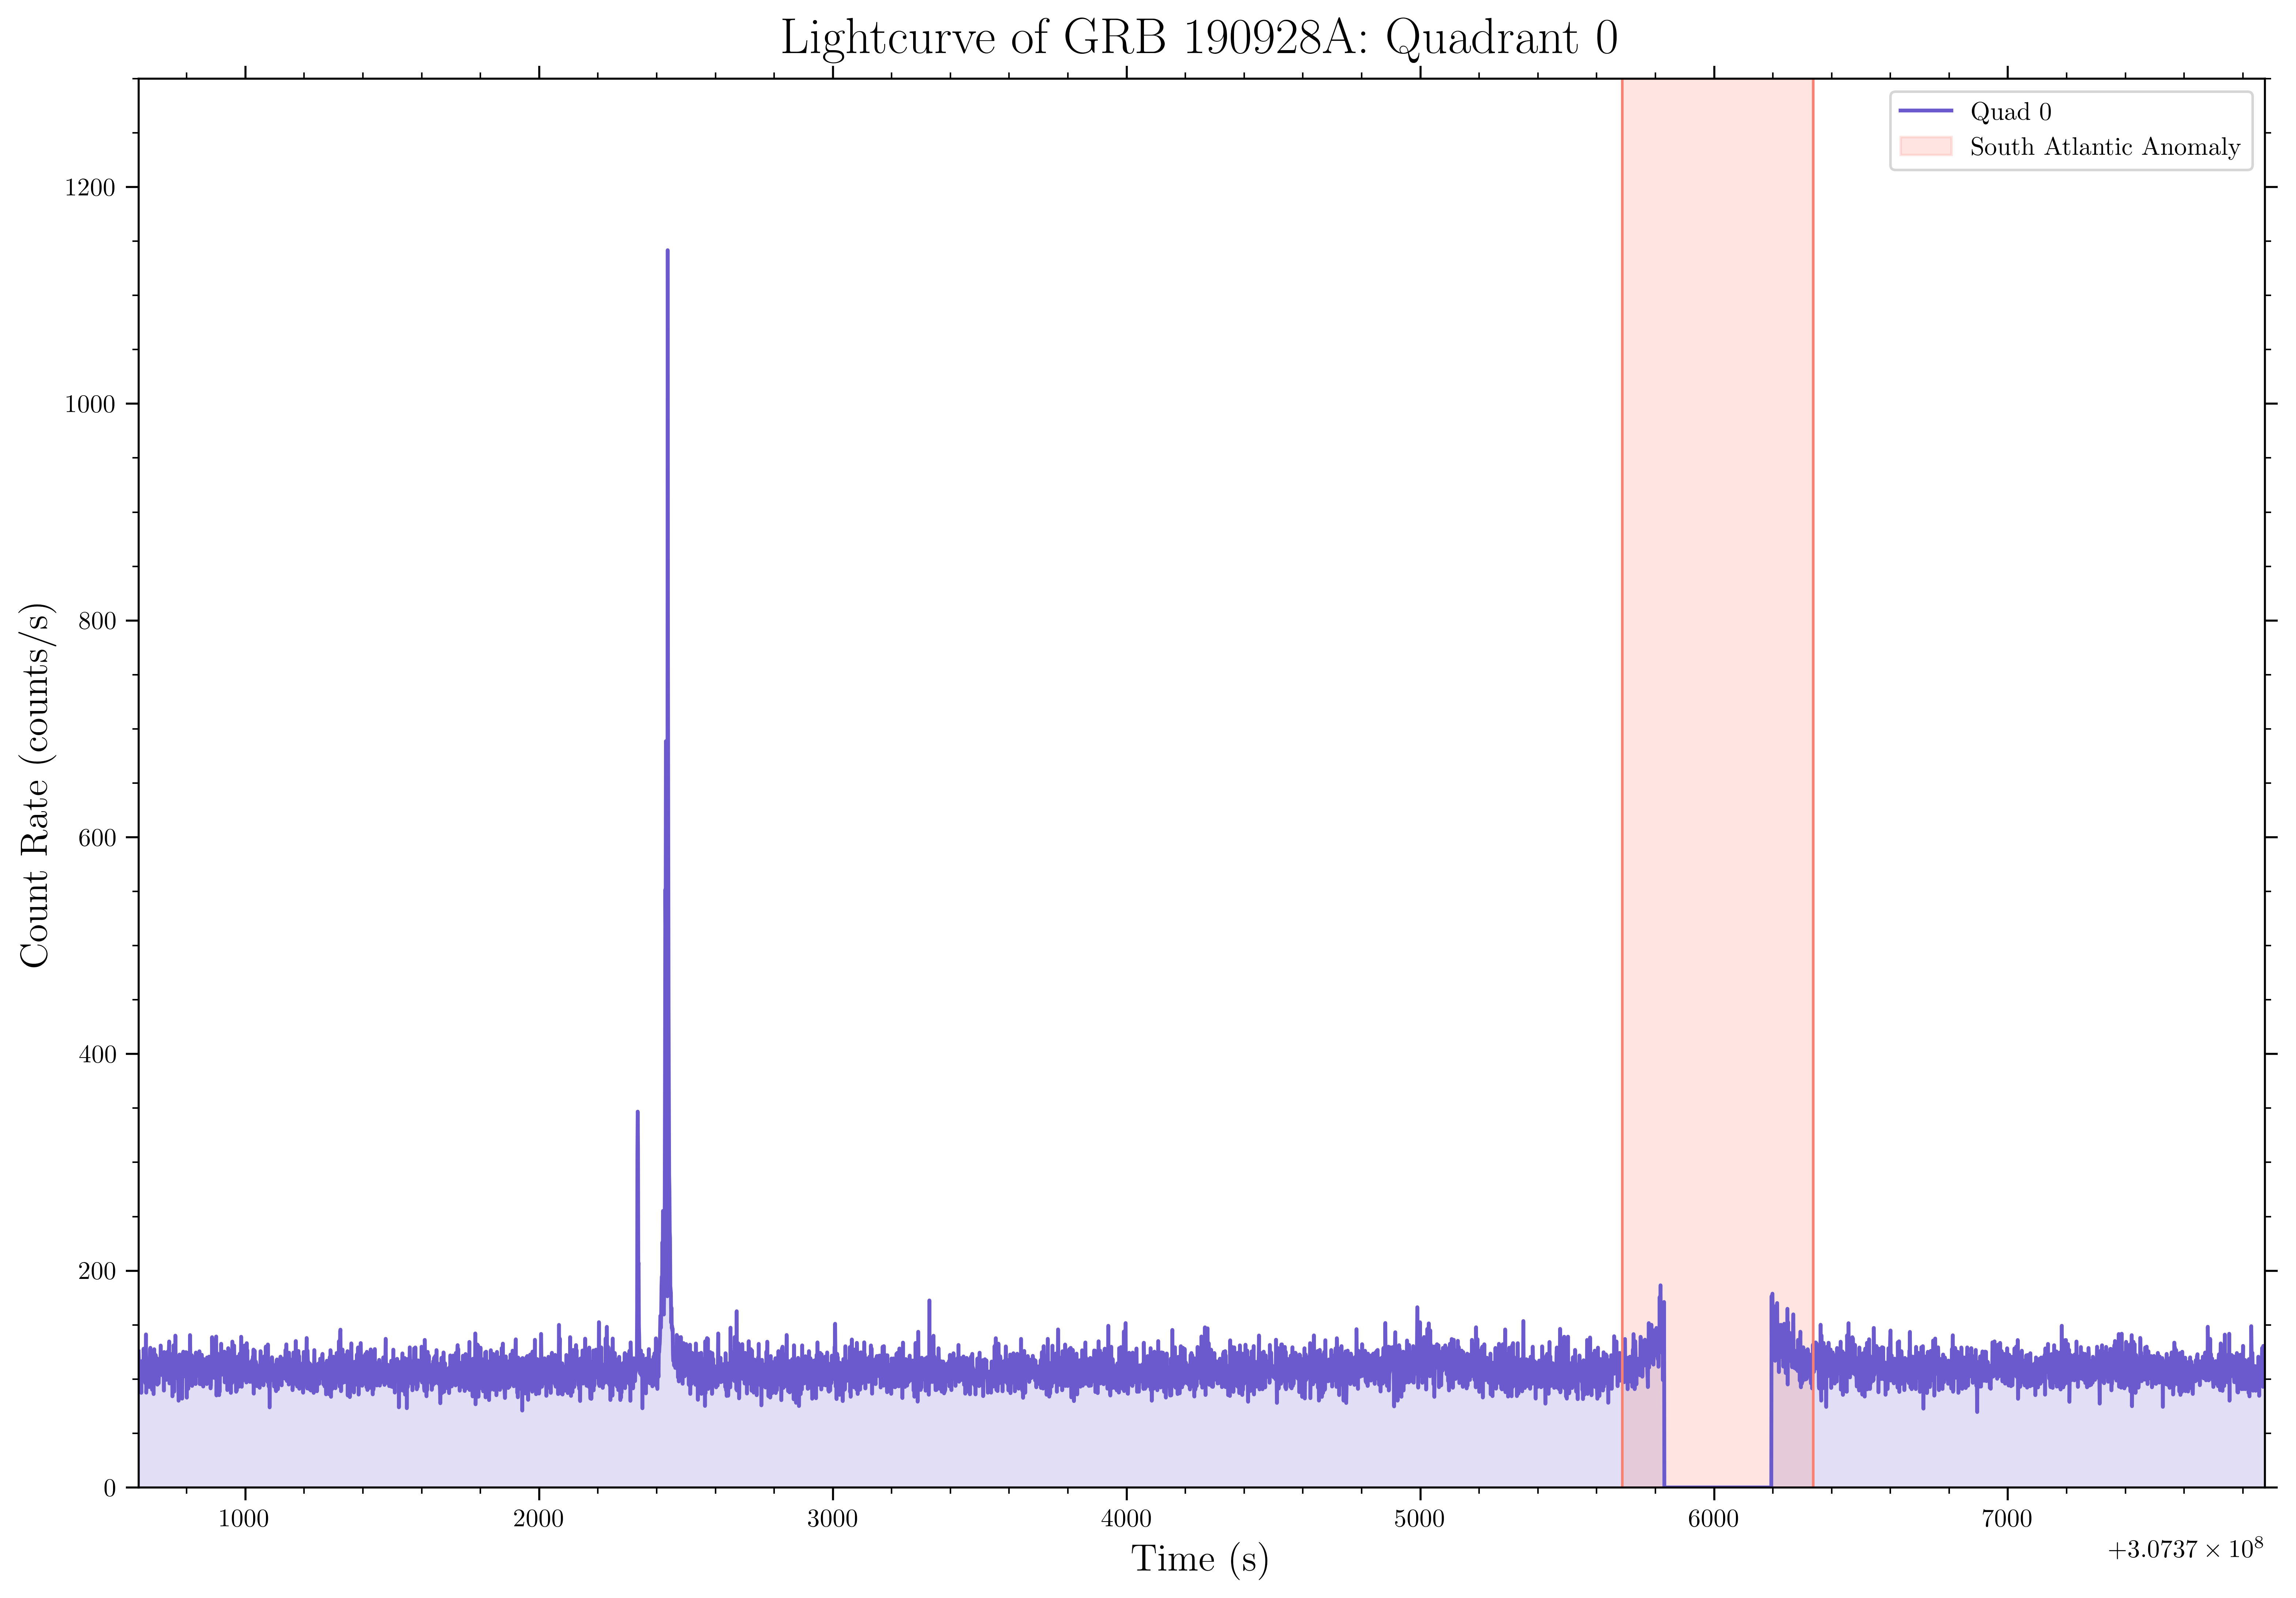
\includegraphics[scale=0.3]{Pictures/anomaly.png}
    \caption{Anomaly in the Light Curve}\label{fig:anomaly}
\end{figure}

The region shaded in red is the region where the counts start rising then fall to 0. This is because there is a high influx of cosmic rays in a particular region in the South Atlantic Ocean. This region is known as the South Atlantic Anomaly (SAA). 

The SAA is a consequence of the fact that the Earth's inner Van Allen radiation belt comes closest to the Earth's surface at the south magnetic pole. This leads to an increased flux of energetic particles in this region and exposes orbiting satellites to higher than usual levels of radiation. 

The detectors on Astrosat are shut off when the satellite passes through the SAA, and hence the counts fall to 0. 

\section{Analysis of GRB190928A}

\subsection{Finding the GRB}

We notice two peaks in the light curve. The first peak is the \href{https://arxiv.org/pdf/1402.7022.pdf}{Prompt Emission}, and the second peak is the \href{https://astronomy.swin.edu.au/cosmos/G/Gamma+ray+burst+afterglow}{Afterglow}. We can find the GRB by looking at the \lstinline[language=Python]{COUNTS} column and finding the maximum value. We can then use the \lstinline[language=Python]{TIME} column to find the time at which the maximum value occurs. In this case, the GRB occurs at 2019-09-28 13:12:17 UTC. 

The duration of the GRB would be the time difference between the time at which the GRB starts and the time at which it ends. The start and end times are taken roughly before the prompt emission and after the afterglow respectively. In this case, the duration of the GRB is 132 seconds.

A thing to note is that \lstinline{cztbindata} produces .lc files for each quadrant of the CZT detectors (namely Quad 0, Quad 1, Quad 2 and Quad 3). We must plot all four quadrants to get a good idea of the GRB.

\begin{figure}[H]
    \centering
    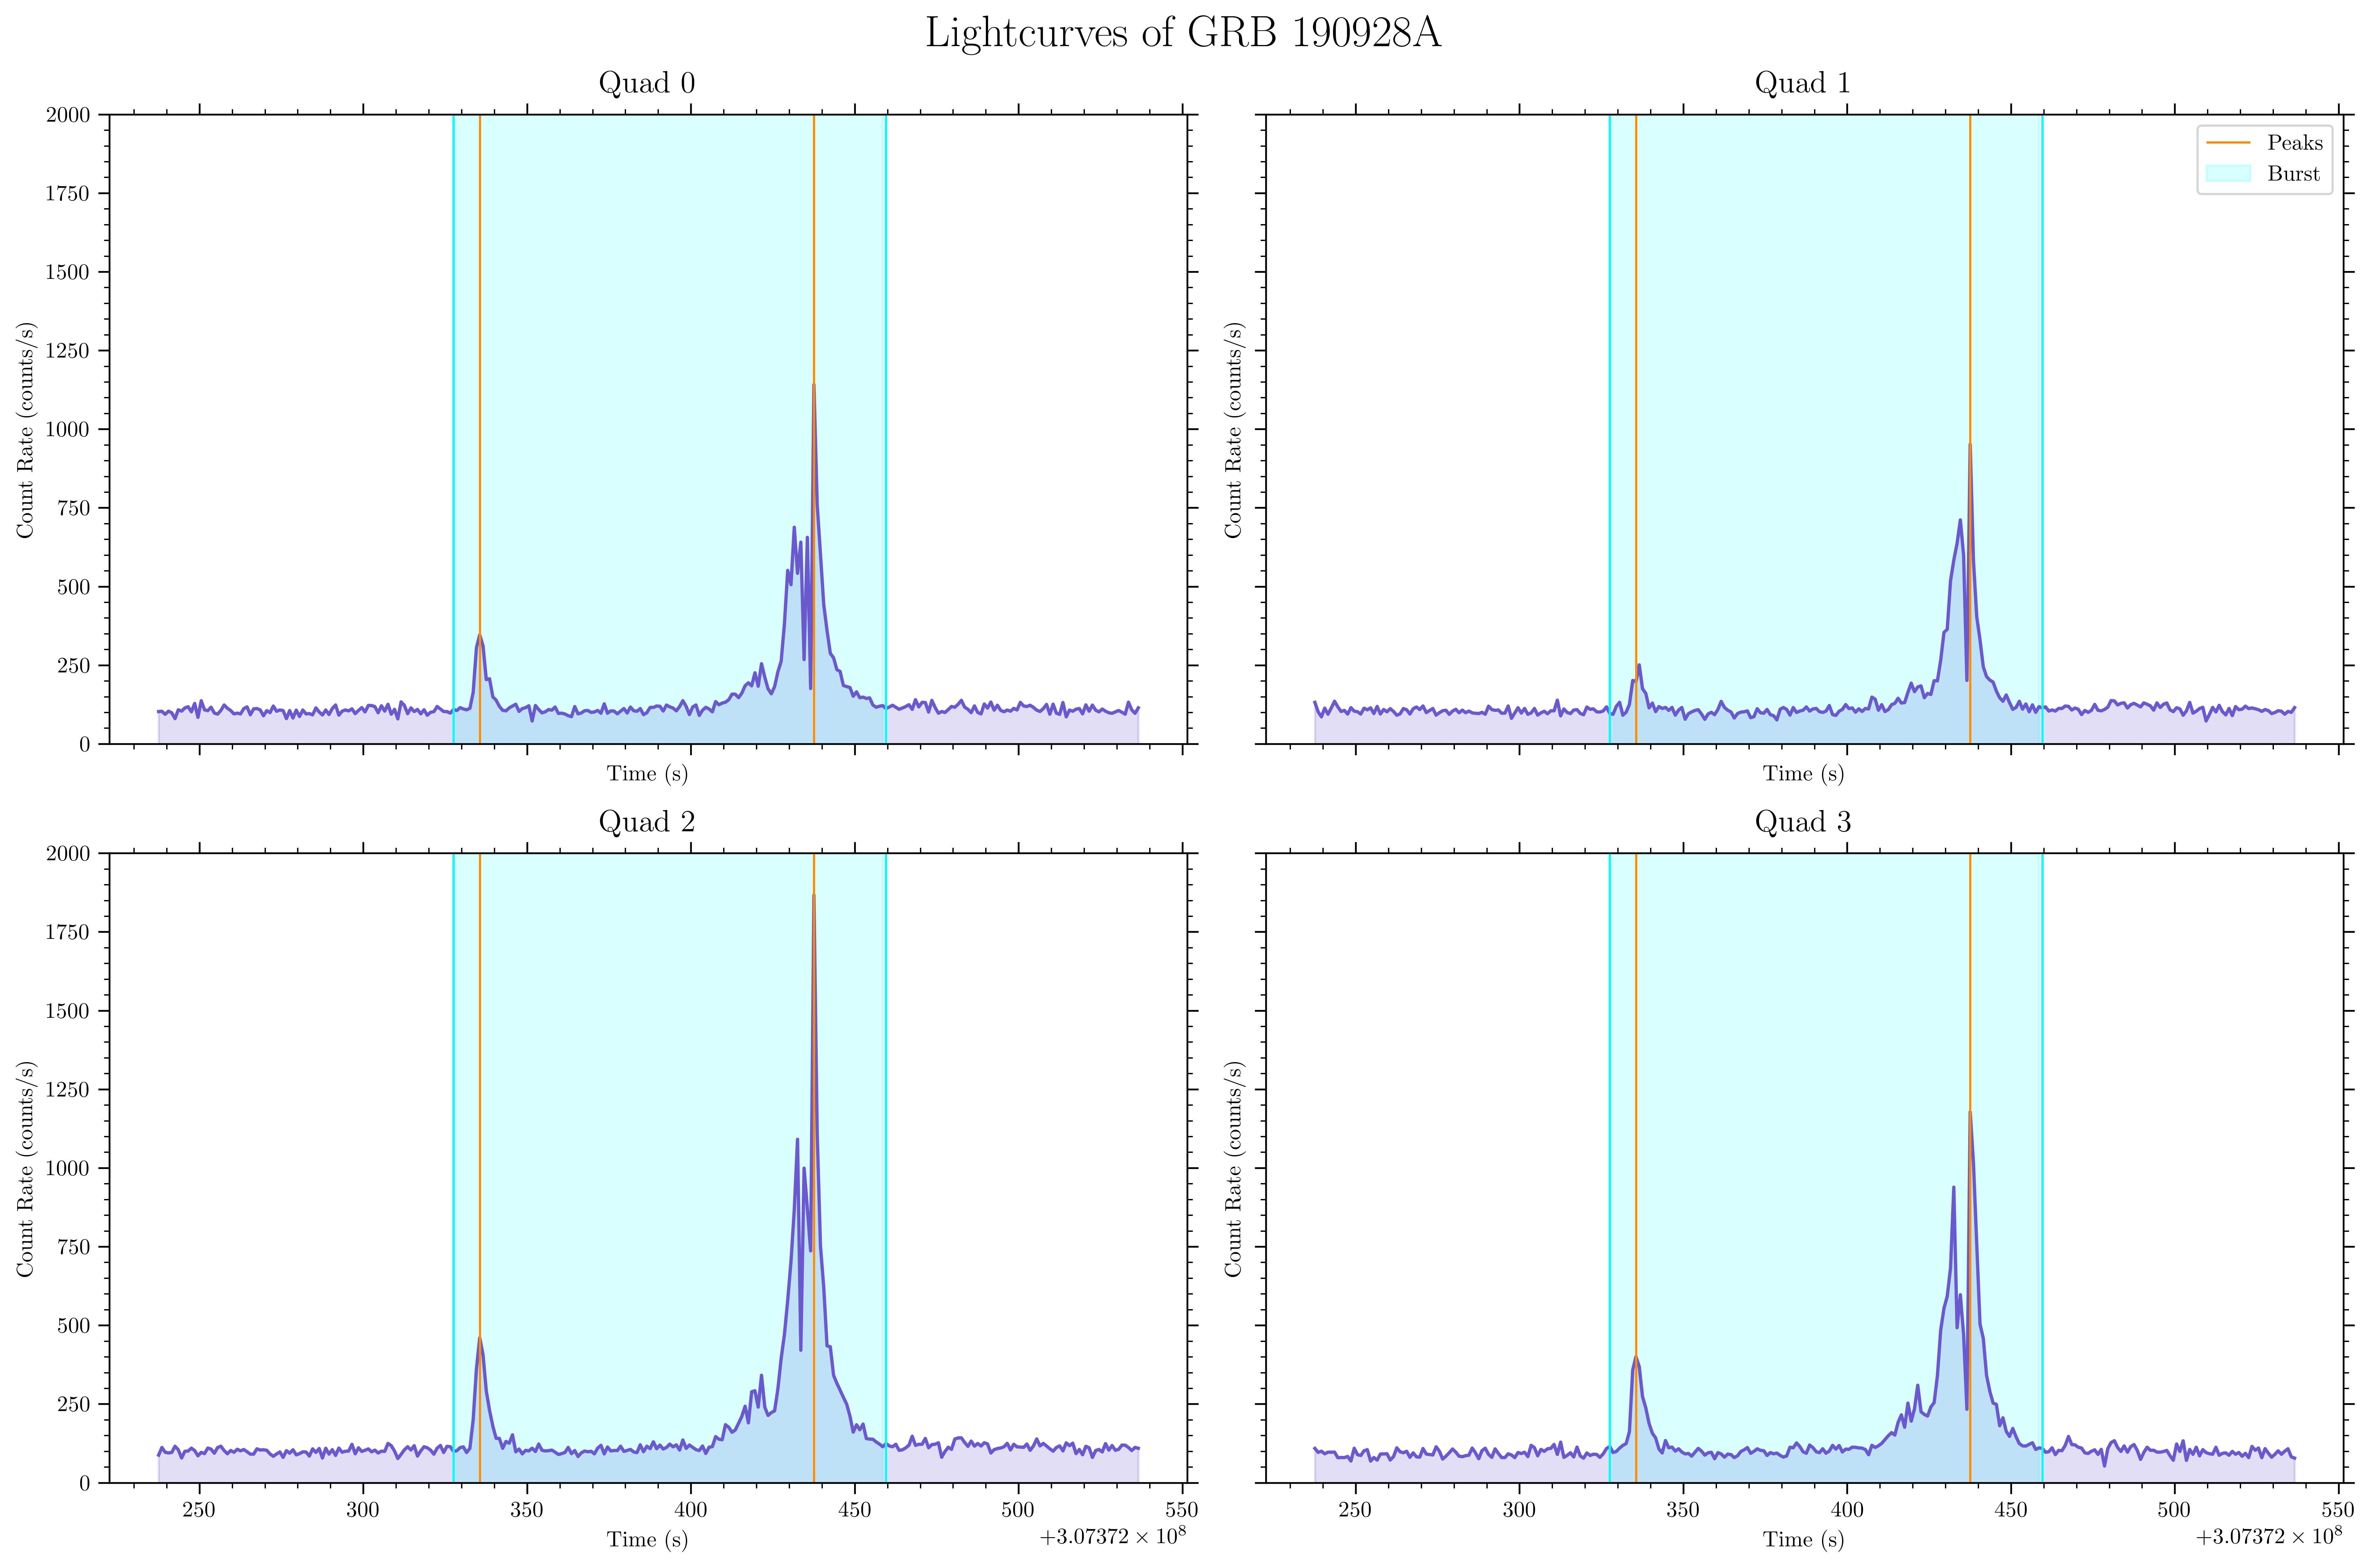
\includegraphics[scale=0.35]{Pictures/allquads.png}
    \caption{Light Curves for all four quadrants}
\end{figure}

The above plot shows the light curves for all four quadrants along with the peaks of the prompt emission and afterglow and markers for the start and end of the GRB.

\subsection{Filtering and Detrending}
%
%
%
% REFER THE FIGURE HERE 
% \ref{fig:anomaly}
%
From Figure \ref{fig:anomaly}, we can see that the "backgorund" data (the signal apart from the GRB) has a mean value somewhere around $100$, along with a lot of variation around that mean value. This variation is known as \textit{noise} and is caused by the inherent physics of the working of the CZTI detectors. There is also an upward slope right before the SAA region which causes a "trend" in the data. We need to "detrend" the data to make any GRB in that region stand out. 

We can do this by using the \lstinline[language=Python]{savgol_filter} function from \lstinline{scipy.stats} to filter the data. The \lstinline[language=Python]{savgol_filter} function applies a \href{https://en.wikipedia.org/wiki/Savitzky%E2%80%93Golay_filter}{Savitzky-Golay filter} to the data. 

The \lstinline[language=Python]{savgol_filter} function takes in the data, the window length and the polynomial order as input. The filter fits a polynomial of a given order to the datapoints in the window, then we subtract this polynomial from the data. This is done for all the datapoints in the window and further for all windows in the data.

The above process is done for the data points \textit{outside} of the GRB region, so as to not detrend the GRB itself. We also have to subtract the mean of the original background ($\approx 100$) from the GRB to get the final GRB data. This step can easily be done before the detrending.

In python, filtering and detrending can be done as follows:

\begin{lstlisting}[language=Python]
    from scipy.signal import savgol_filter
    import numpy as np
    # Subtracting the mean of the original background
    data[grb] -= np.mean(data[grb])
    # Filtering and Detrending
    data[noise] -= savgol_filter(data[noise], 101, 3)
\end{lstlisting}

\begin{wrapfigure}{l}{0.7\textwidth}
    \centering
    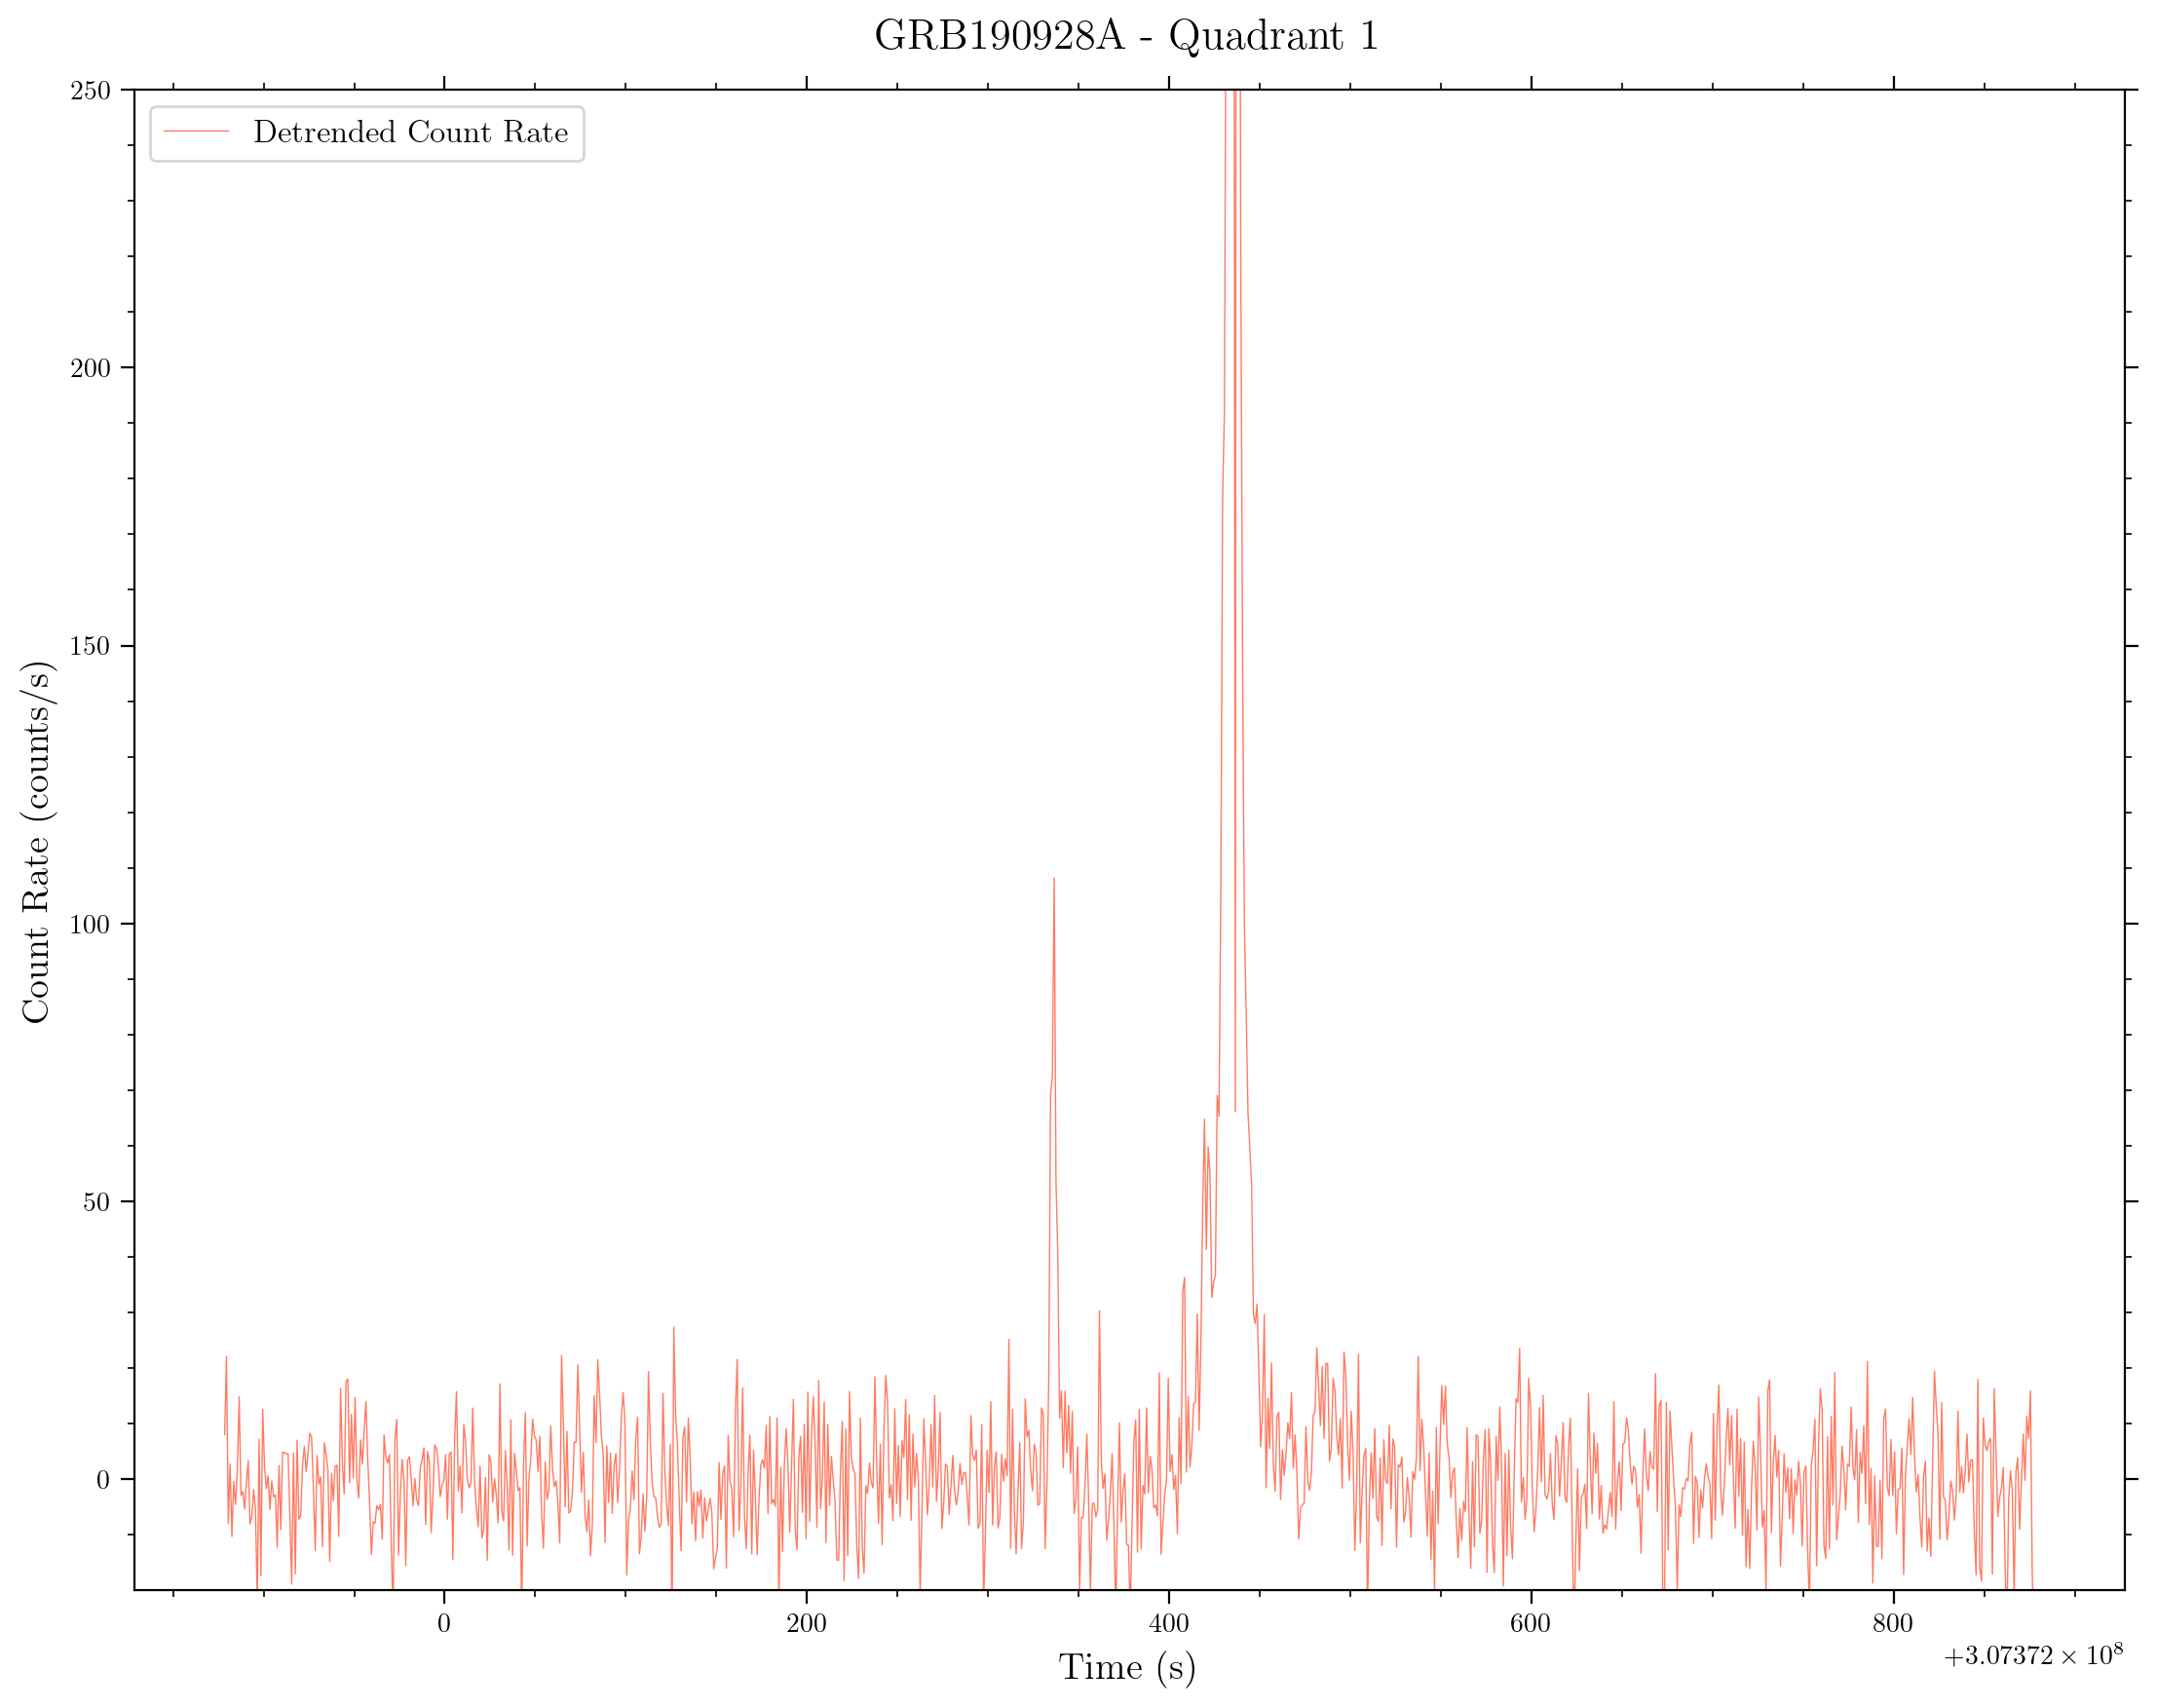
\includegraphics[scale=0.25]{Pictures/detrended.png}
    \caption{Detrended Light Curve}
\end{wrapfigure}


For the purposes of our analysis, we will be using a window length of $101$s and a polynomial order of $3$. The results of the filtering and detrending are shown below:

To the left we can see that the slope next to the SAA region has been removed, the background has been reduced to nearly $0$, and the GRB has been brought down from the original background of $\approx 100$ to $\approx 0$.

We can also see that the "dip" that occurs during the SAA region is now a flat line with values equal to $0$.

\clearpage

\section{Different Bin Sizes}

Uptil now we have analysed the data using a bin size of $1$s. We can also analyse the data using different bin sizes to see how the results change. For the purposes of this analysis, we will be using bin sizes of $0.1$s, $1$s, $10$s.

\begin{figure}[H]
    \centering
    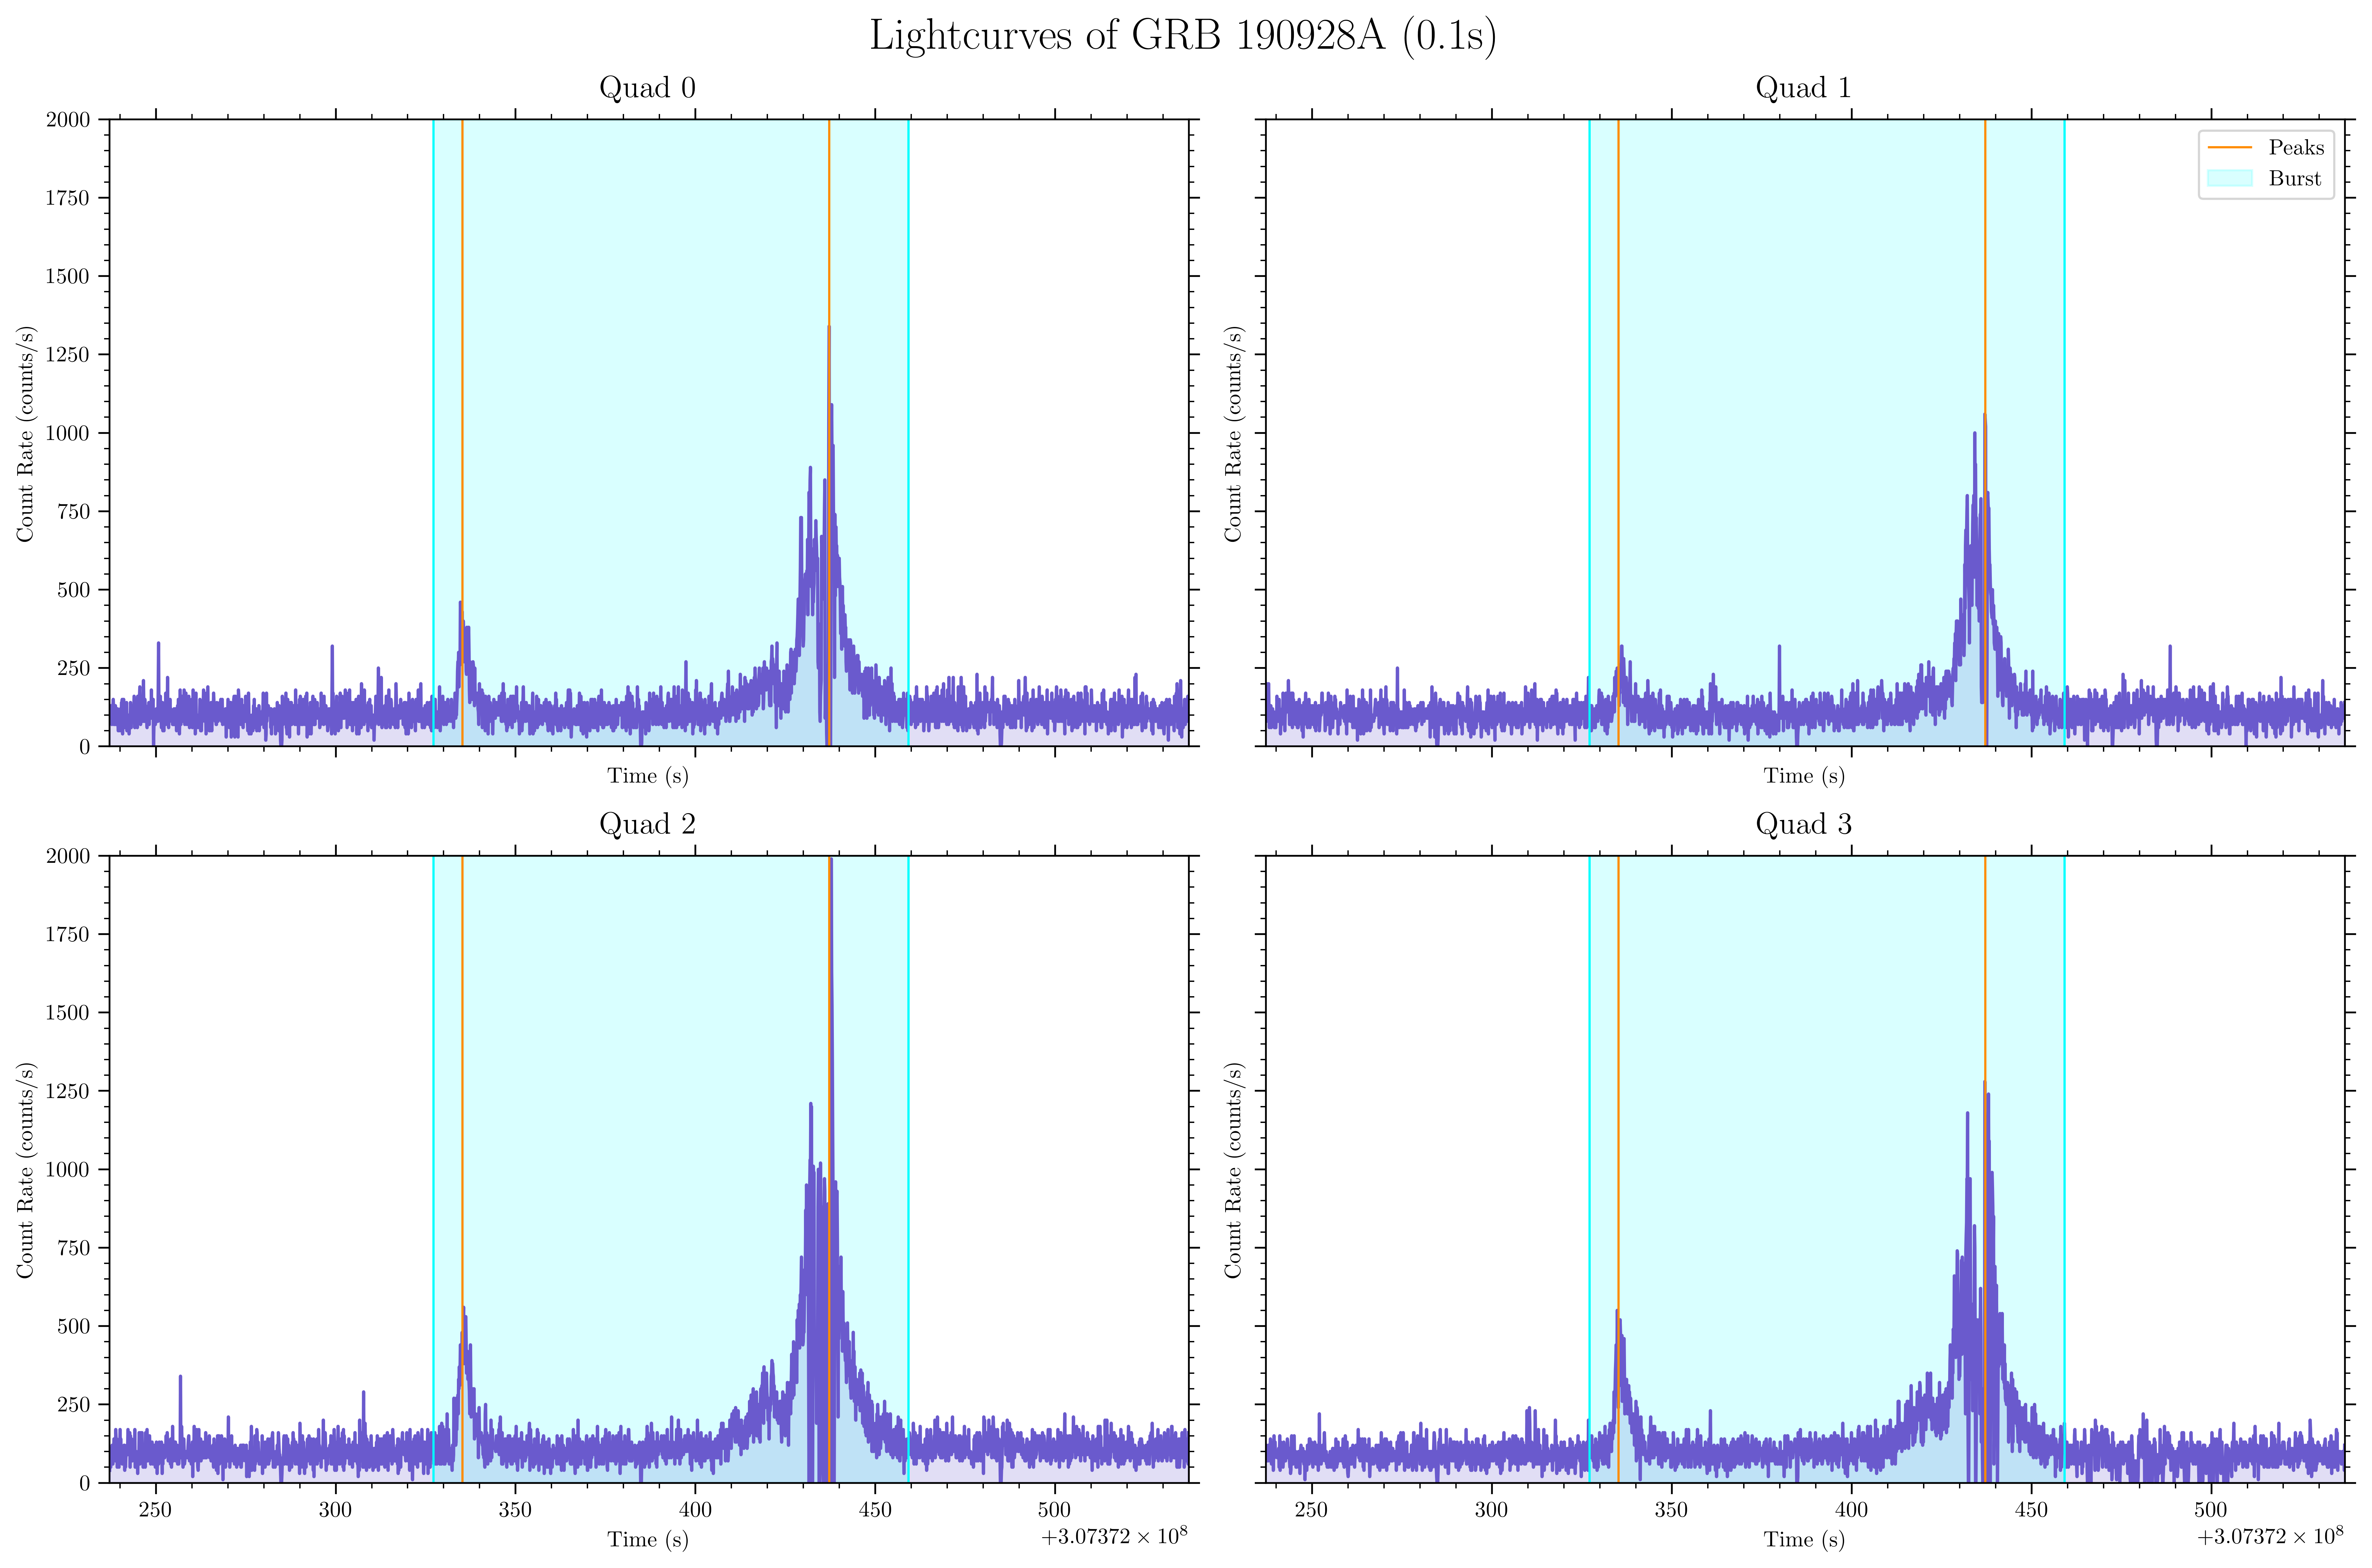
\includegraphics[width=0.8\textwidth]{Pictures/allquads01s.png}
    \caption{Light Curves for bins of 0.1s}
    \label{fig:smallbins}
\end{figure}

Here we have the light curves of all four quadrants during the interval of the GRB. We can see that the smaller binsize causes the variations in the background to be more prominent. 

\begin{figure}[H]
    \centering
    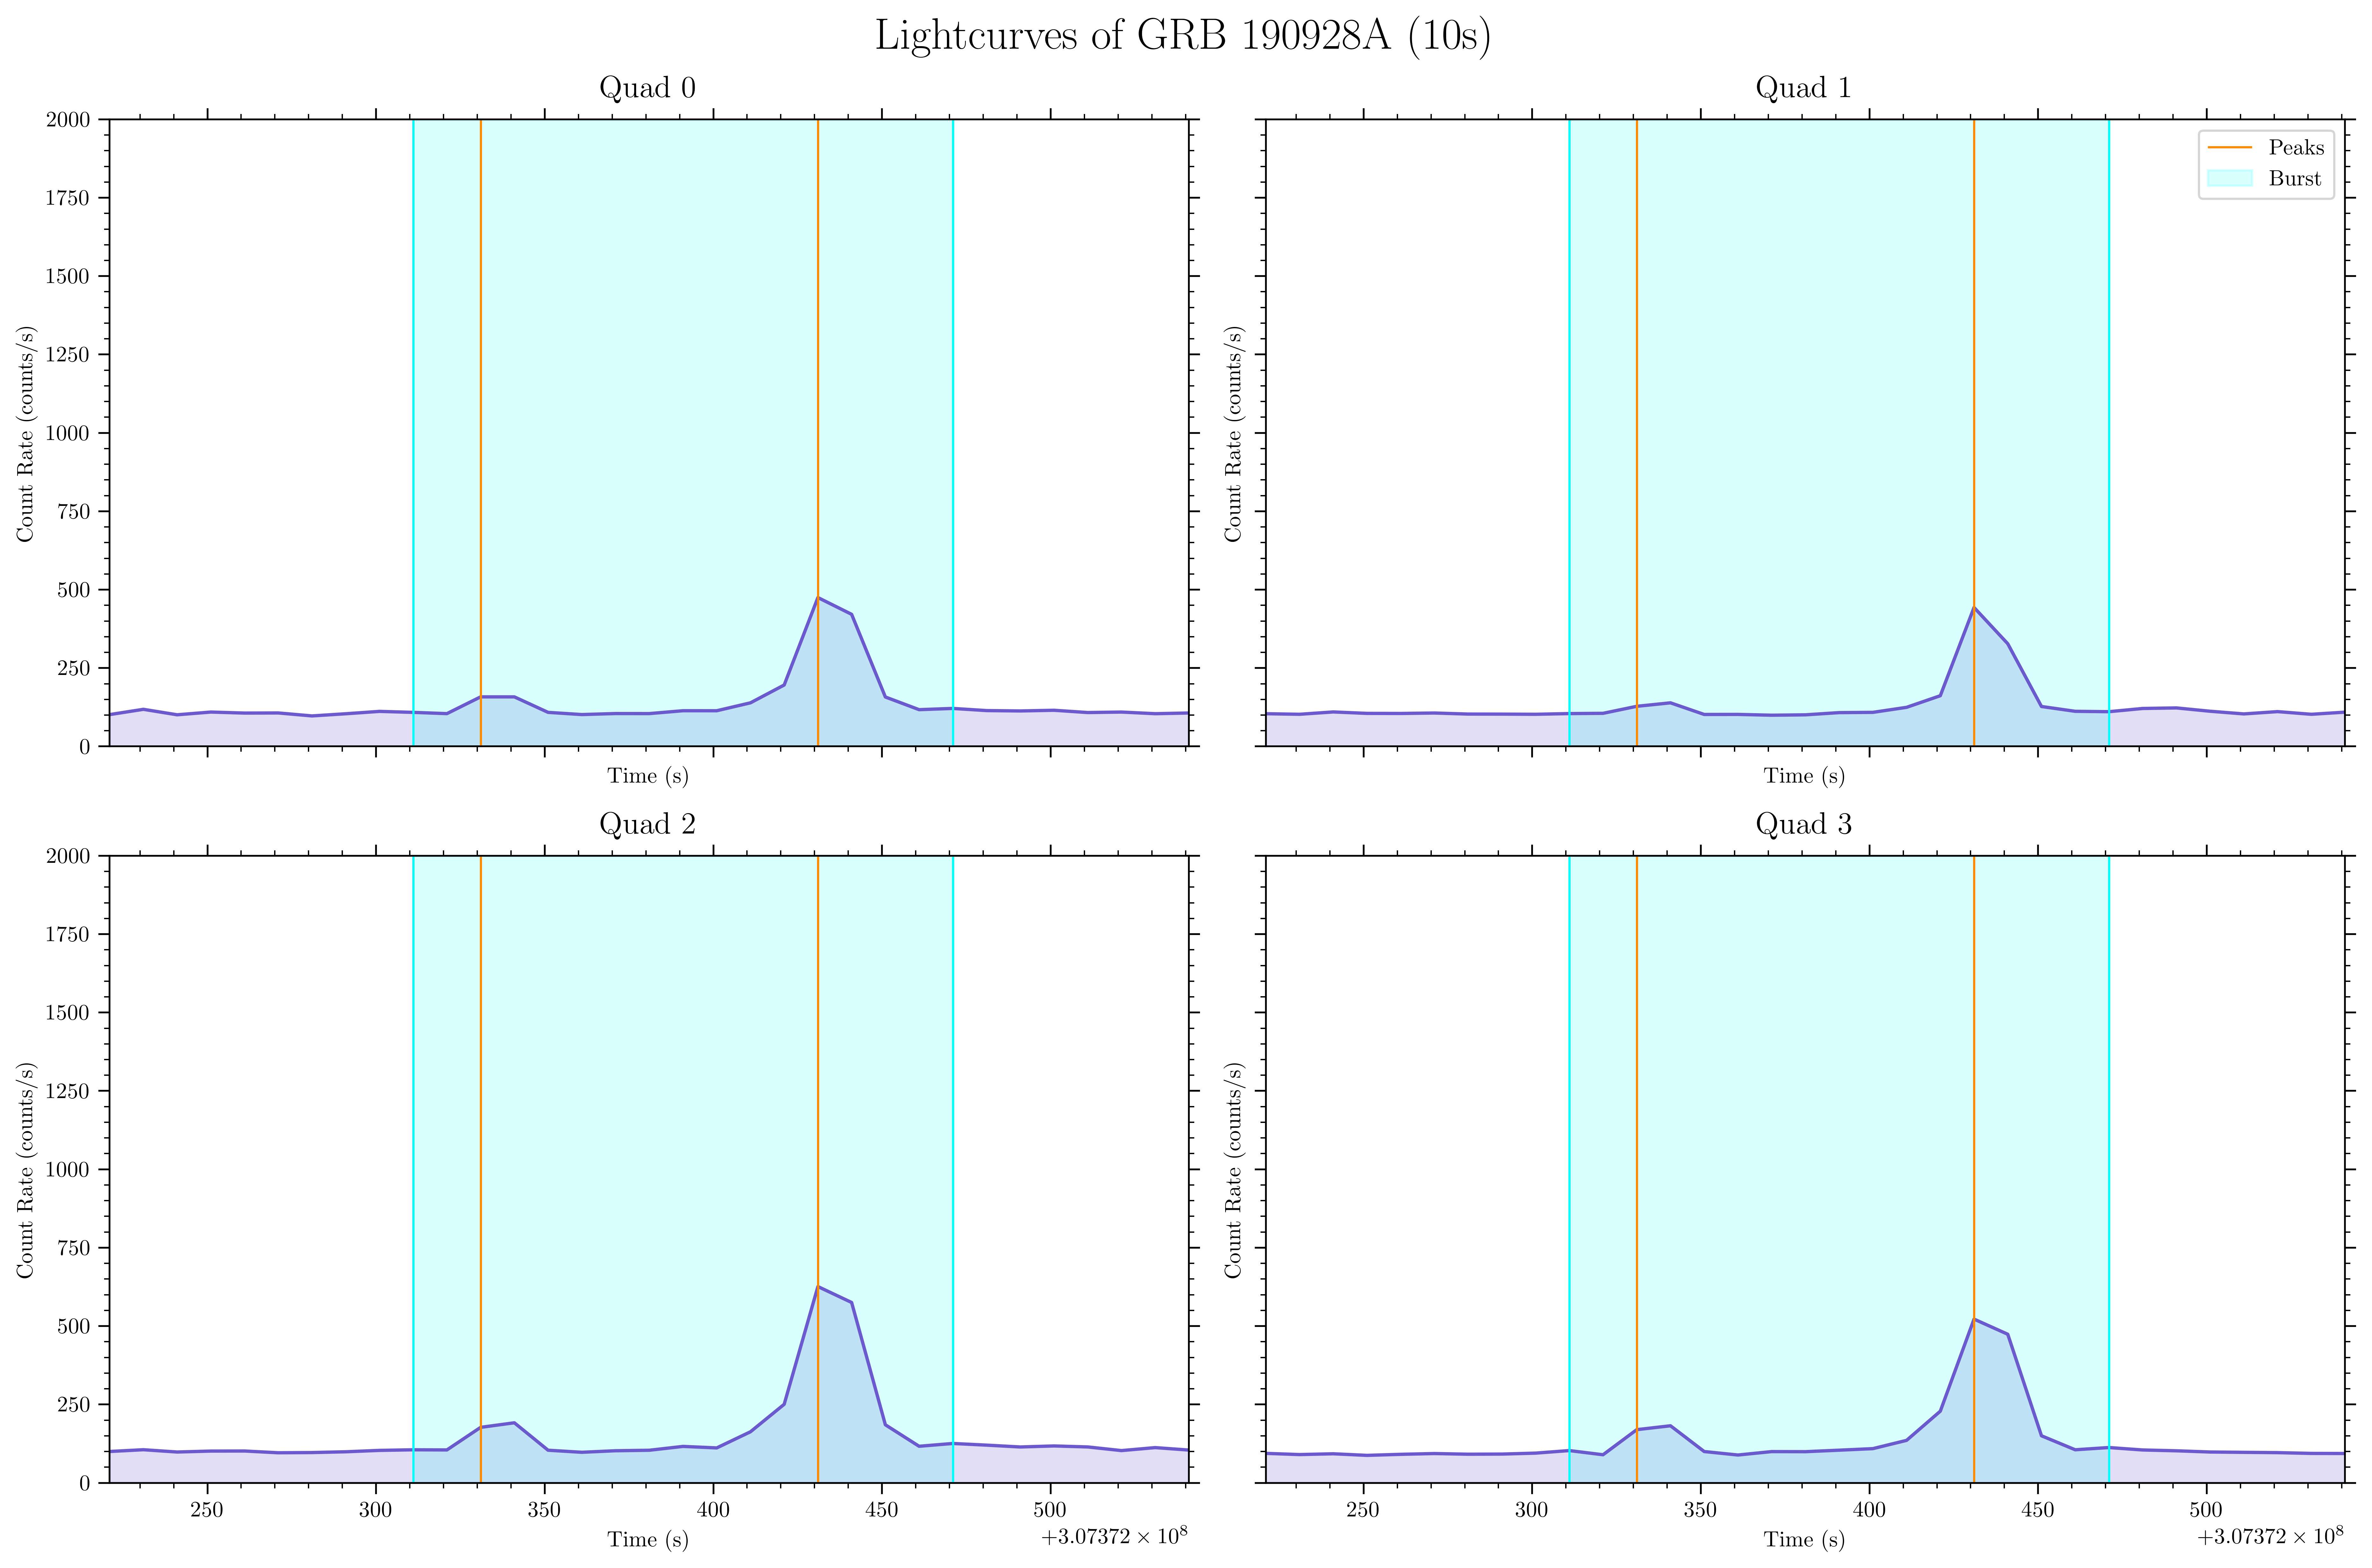
\includegraphics[width=0.8\textwidth]{Pictures/allquads10s.png}
    \caption{Light Curves for bins of 10s}
\end{figure}

Here we can see that the larger binsize causes the variations in the background to be less prominent, as more of the noise gets smooothened (averaged) out.


%----------------------------------------------------------------------------------------
%	CHAPTER 3
%----------------------------------------------------------------------------------------
\chapterimage{lgm.png}
\chapter{Signal To Noise Ratio}

\section{Introduction}

The signal-to-noise ratio (SNR) is a measure used in science and engineering that compares the level of a desired signal to the level of background noise. SNR is defined as the ratio of signal power to the noise power, often expressed in decibels. A ratio higher than 1:1 (greater than 0 dB) indicates more signal than noise. While SNR is commonly quoted for electrical signals, it can be applied to any form of signal, in out case, we will be finding the SNR of a single in a timeseries. 

%
% REFER THE FIGURE HERE
% \ref{fig:smallbins}

Now, comparing the levels of the signal and noise are easier said than done. The signal is the GRB, and the noise is the background. The background is not constant, and varies a lot. This particular variation can be seen most clearly in Figure \ref{fig:smallbins}. GRB 190928A is a particularly bright GRB, so it is easy to see the GRB in the light curve. But what about fainter GRBs? How do we find the SNR of a faint GRB? We'll look at the various methods used to determine the SNR in the upcoming sections.


\subsection{Methodology}
There are a plethora of methods that can be used to determine the SNR of a GRB. There are methods that involve integrating the signal and noise separately and then dividing the two, there are methods that involve fitting a distribution to the noise and taking a certain percentile of the distribution as the noise and so on. Regardless of the methods, the crux of the matter is to find quantities that best describe the signal and the noise.

\newpage

\section{Signal}

Describing the signal is a fairly straightforward task as opposed to describing the noise.

The signal is the GRB, and the GRB is a peak in the light curve. So, we can describe the signal as the maximum value of the light curve textit{in the GRB window}. This is the simplest way of describing the signal, and is the method we will be using for the majority of this project and will be referred to as \textbf{$M_s$}.

Another method of describing the signal is to integrate the light curve over the duration of the GRB. This method will be taken as a baseline for the other methods.

\section{Noise}

Describing the noise is a much more difficult task than describing the signal. The noise is the background, and the background is not constant. The background varies a lot, and the variation is slightly different for each orbit of the satellite, as well as each quadrant of the CZT detectors.

\subsection{Method 1 - Time Averaged Integrals}
Since we are dealing with data that is already time binned, our "Integral" simply becomes the sum of the counts for both the noise and the signal. An important thing to note is that the duration of the GRB is not the same as the duration of the we sample from the lightcurve, so it's important to normalise the values of the signal and noise by dividing by their respective durations.

Mathematically speaking, we can write this down as: 

\begin{align*}
    \text{Signal} = \frac{\sum_{i=0}^{n} \text{Counts}_i}{\text{Duration of GRB}} 
    &&
    \text{Noise} = \frac{\sum_{i=0}^{m} \text{Counts}_i}{\text{Duration of Noise}}
\end{align*}
    
Where $n$ is the number of data points in the GRB, and $m$ is the number of data points in the noise.

\subsection{Method 2 - Fitting a Distribution to the Noise} \label{sec:method2}

This method involves fitting a distribution to the noise and then taking a certain sigma clip of the distribution as the noise. This method is more robust than the previous method as it takes into account the variation in the noise. Say for example, the noise is a Gaussian distribution, then we fit a Gaussian distribution by varying the mean ($\mu$) and standard deviation ($\sigma$) till we get the best fit. We then take the value of noise as $\mu+3\sigma$. 

There are quite a few different distributions that are of interest to us, namely the Gaussian, Poisson, Gamma, Weibull and Rayleigh distributions. We will be looking at each of these distributions and the troubles faced in fitting them in the upcoming sections.

\textit{\textbf{An important note:} When we fit the noise to some distrbution, according to the nature of the distribution, we get a value for the optimal mean and standard deviation that will fit our noise. Since the data has been detrended, our noise is centered around $0$, so our entire data must be shifted by the mean obtained by fitting, and our signal becomes \textbf{$M_s+\mu$.}}


\newpage

\subsection{Gaussian Distribution}

A Gaussian distribution is a continuous function representing the distribution of many random variables as a symmetrical bell-shaped graph. The Gaussian distribution is also known as the normal distribution. The equation for a Gaussian distribution is given by:

\begin{equation} \label{eq:gaussian}
    f(x) = \tfrac{1}{\sigma\sqrt{2\pi}}e^{-\tfrac{(x-\mu)^2}{2\sigma^2}}
\end{equation}

Where $\mu$ is the mean and $\sigma$ is the standard deviation of the distribution. The Gaussian is of some interest to us because the noise in the light curves follows a rough bell-shaped distribution. 

Fitting a Gaussian is pretty straight forward using the \lstinline[language=Python]{scipy.optimize.curve_fit} function, and defining a function that produces a purely Gaussian equation either by using the equation (\ref{eq:gaussian}) or the \lstinline[language=Python]{scipy.stats.norm.pdf} function. In either case, the function takes in the data as input and returns the mean and standard deviation of the distribution. 

We can then take the noise as $\mu+3\sigma$ and the signal as $M_s+\mu$ (Recall the note at the end of Section \ref{sec:method2}).

\begin{equation}
    \therefore \text{SNR} = \frac{M_s+\mu}{\mu+3\sigma}
\end{equation}

\begin{figure}[H]
    \centering
    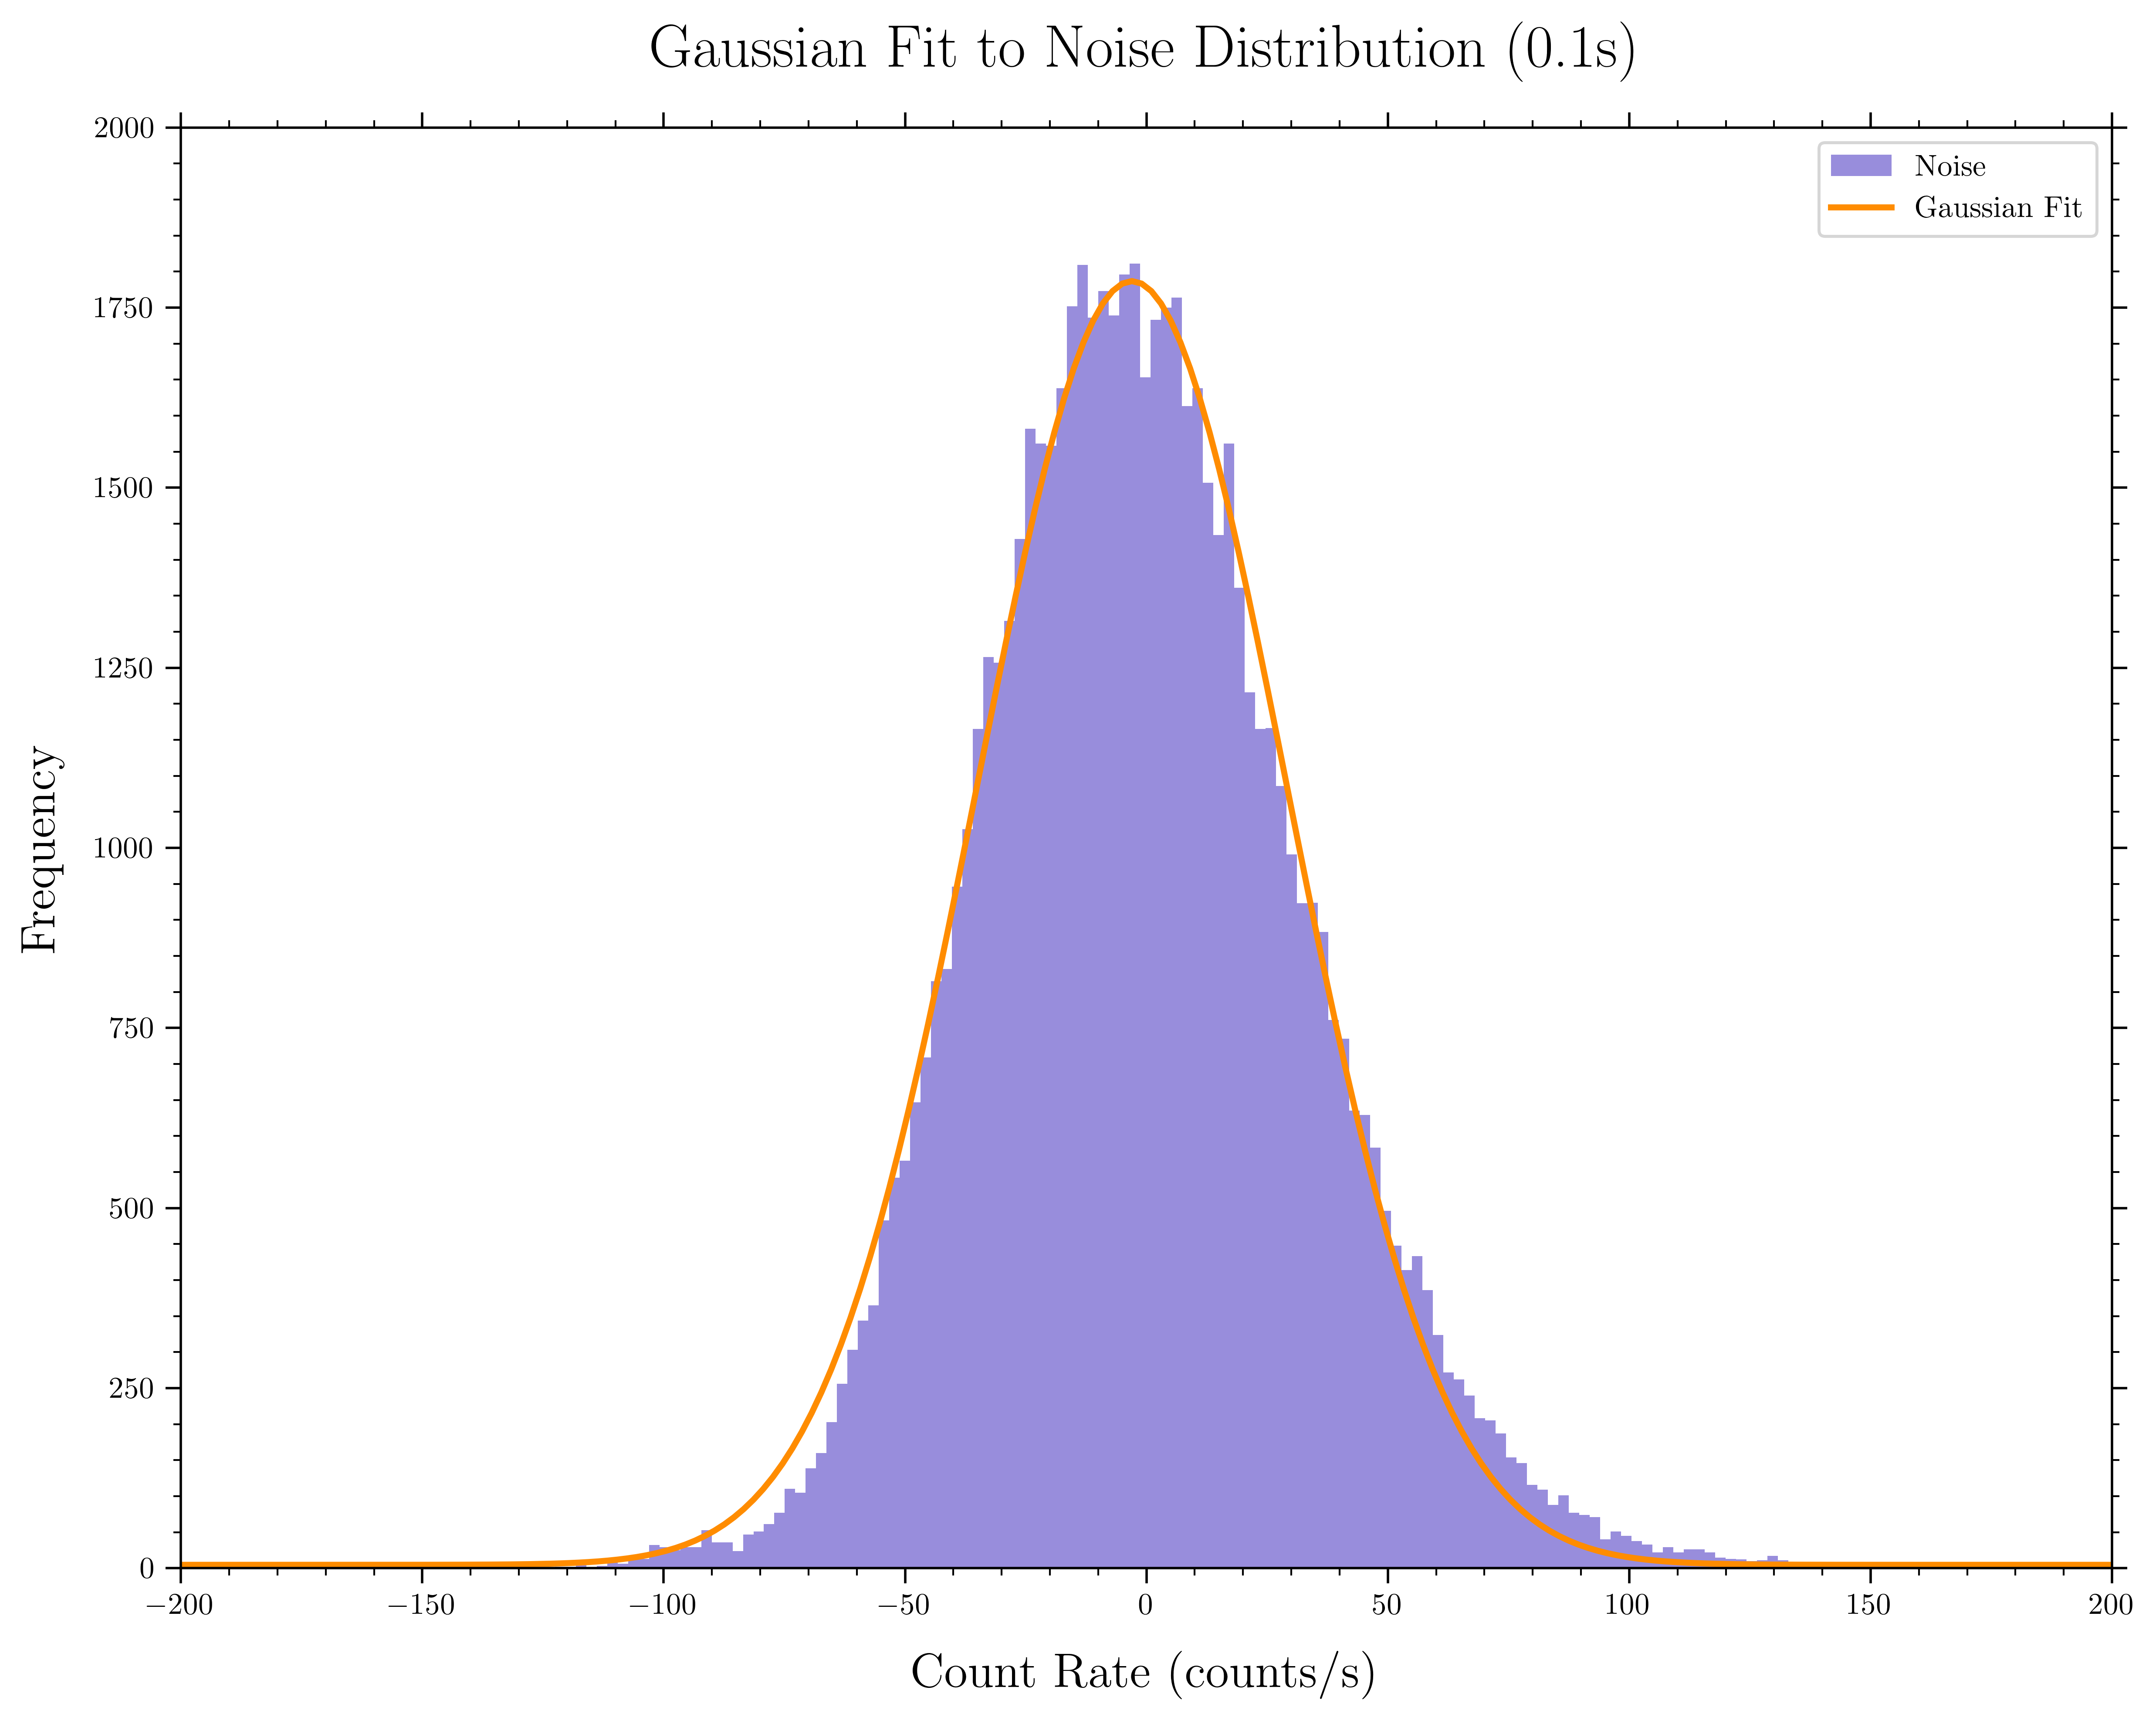
\includegraphics[width=0.8\textwidth]{Pictures/gaussian_fit.png}
    \caption{Fitting a Gaussian to the Noise (BinSize 0.1s) of Quadrant 0}
\end{figure}

It's clear from the above picture that our noise is \textit{not} Gaussian but a Gaussian is a good approximation of the noise.


\subsection{Poisson Distribution}

The Poisson distribution is a discrete probability distribution that expresses the probability of a given number of events occurring in a fixed interval of time or space if these events occur with a known constant mean rate and independently of the time since the last event. The Poisson distribution can also be used for the number of events in other specified intervals such as distance, area or volume. The Poisson distribution is defined as:

\begin{equation} \label{eq:Poisson}
    f(k; \lambda)=\frac{\lambda^k e^{-\lambda}}{k!}
\end{equation}
    
Where $k$ is the number of events, and $\lambda$ is the average number of events per interval. An interesting thing to note is that the mean and variance of the Poisson distribution are both equal to $\lambda$. The Poisson distribution is of interest to us because the noise in the light curves seems to have a skewed distribution, and the Poisson distribution, in general, approximates a skewed distribution well.

Fitting a Poisson distribution is a bit more complicated than fitting a Gaussian distribution. We use the \lstinline[language=Python]{scipy.optimize.curve_fit} function and defining a function that returns a Poisson distribution by using \lstinline[language=Python]{scipy.stats.poisson.pmf}. In this case we obtain only the mean of the distribution ($\lambda$). 

We can now take the noise as $\lambda+3\sqrt{\lambda}$ and the signal as $M_s+\lambda$. 

\begin{equation}
    \therefore \text{SNR} = \frac{M_s+\lambda}{\lambda+3\sqrt{\lambda}}
\end{equation}

\begin{figure}[H]
    \centering
    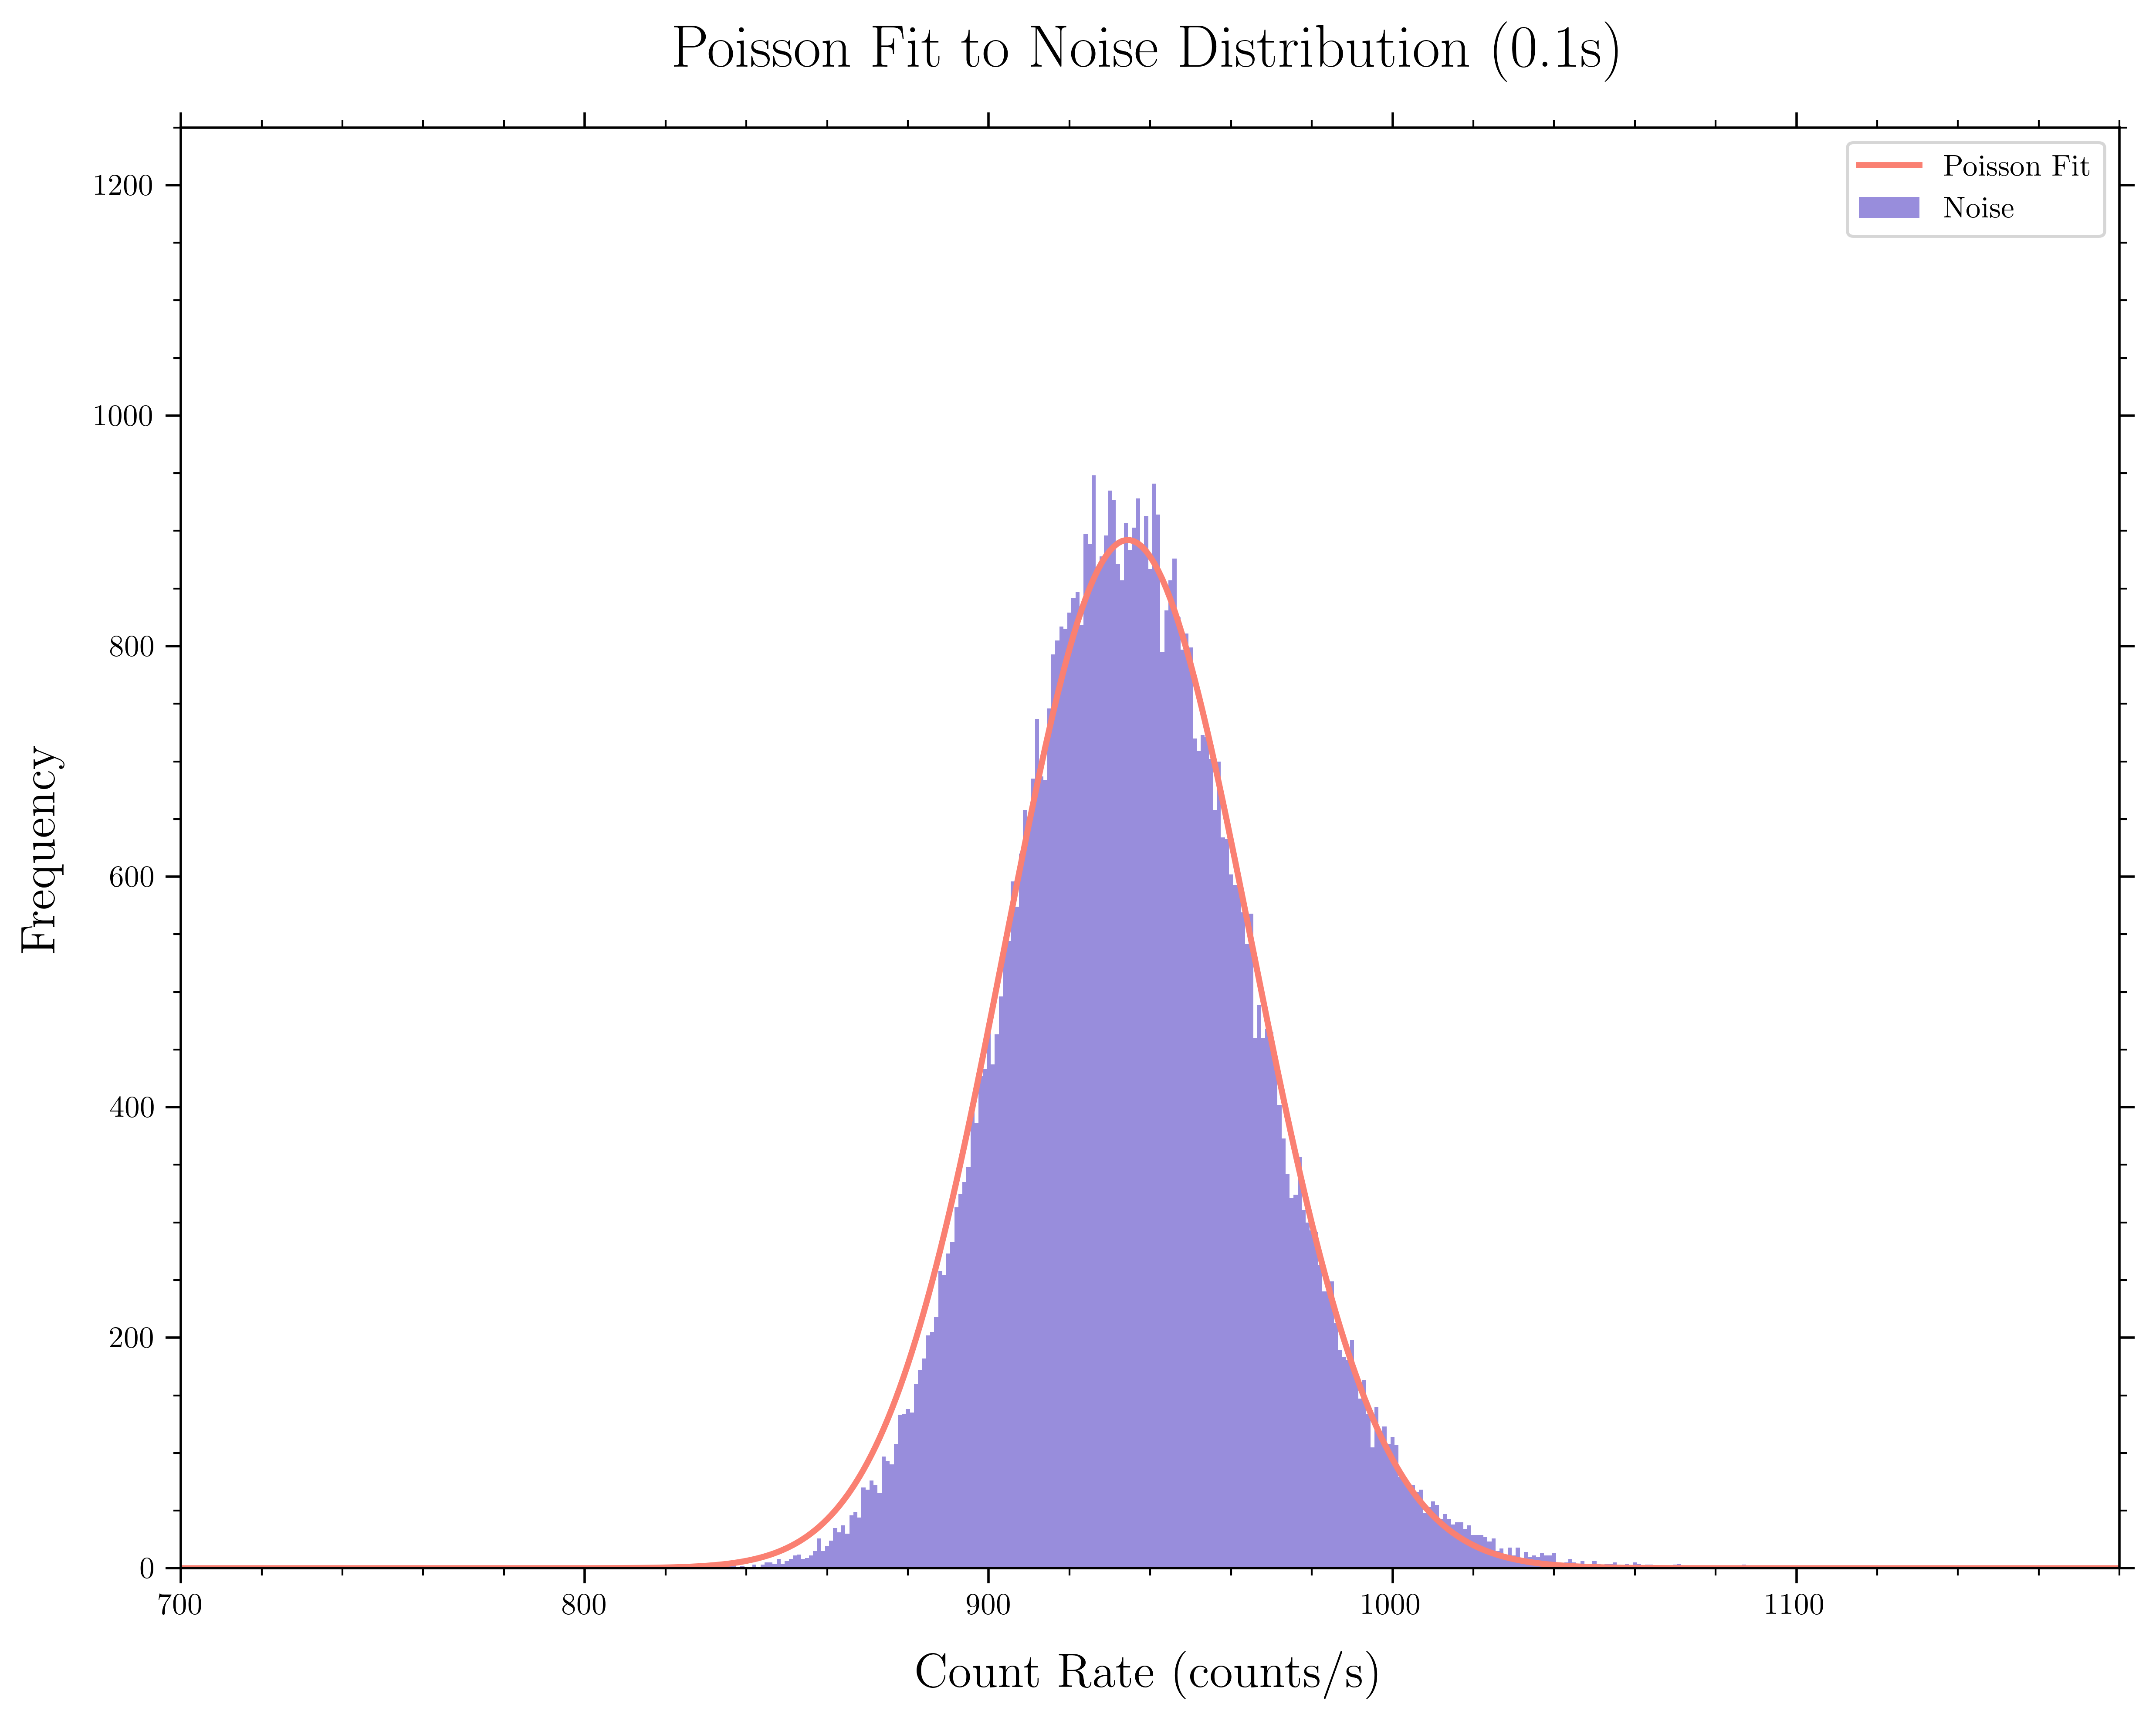
\includegraphics[width=0.8\textwidth]{Pictures/poisson_fit.png}
    \caption{Fitting a Poisson Distribution to the Noise (BinSize 0.1s) of Quadrant 0}
\end{figure}

We can see that the Poisson distribution is a better fit to the noise than the Gaussian distribution.


\subsection{Gamma Distribution}

The Gamma distribution is a two-parameter family of continuous probability distributions. The exponential distribution, Erlang distribution, and chi-squared distribution are special cases of the Gamma distribution. There are two different parameterisations in common use:

\begin{itemize}
    \item With a shape parameter $k$ and a scale parameter $\theta$.
    \item With a shape parameter $\alpha = k$ and an inverse scale parameter $\beta = 1/\theta$, called a rate parameter.
\end{itemize}

In either case, the probability density function of the Gamma distribution is given by:

\begin{equation} \label{eq:Gamma}
    f(x; k, \theta) = \frac{x^{k-1}e^{-x/\theta}}{\theta^k\Gamma(k)}
\end{equation}
    
    Where $\Gamma(k)$ is the Gamma function, and the mean is given by $k\theta$ and variance is $k\theta^2$. The Gamma distribution is of interest to us because the noise in the light curves seems to have a skewed distribution, and the Gamma distribution can also approximate a skewed distribution well.

Fitting a Gamma distribution is a bit simpler than fitting a Poisson distribution. We use the \lstinline[language=Python]{scipy.stats.gamma.fit} function that can directly give us the shape and scale parameters of the distribution.

We can now take the noise as $k\theta + 3\sqrt{k\theta^2}$ and the signal as $M_s+k\theta$.

\begin{equation}
    \therefore \text{SNR} = \frac{M_s+k\theta}{k\theta + 3\sqrt{k\theta^2}}
\end{equation}

\begin{figure}[H]
    \centering
    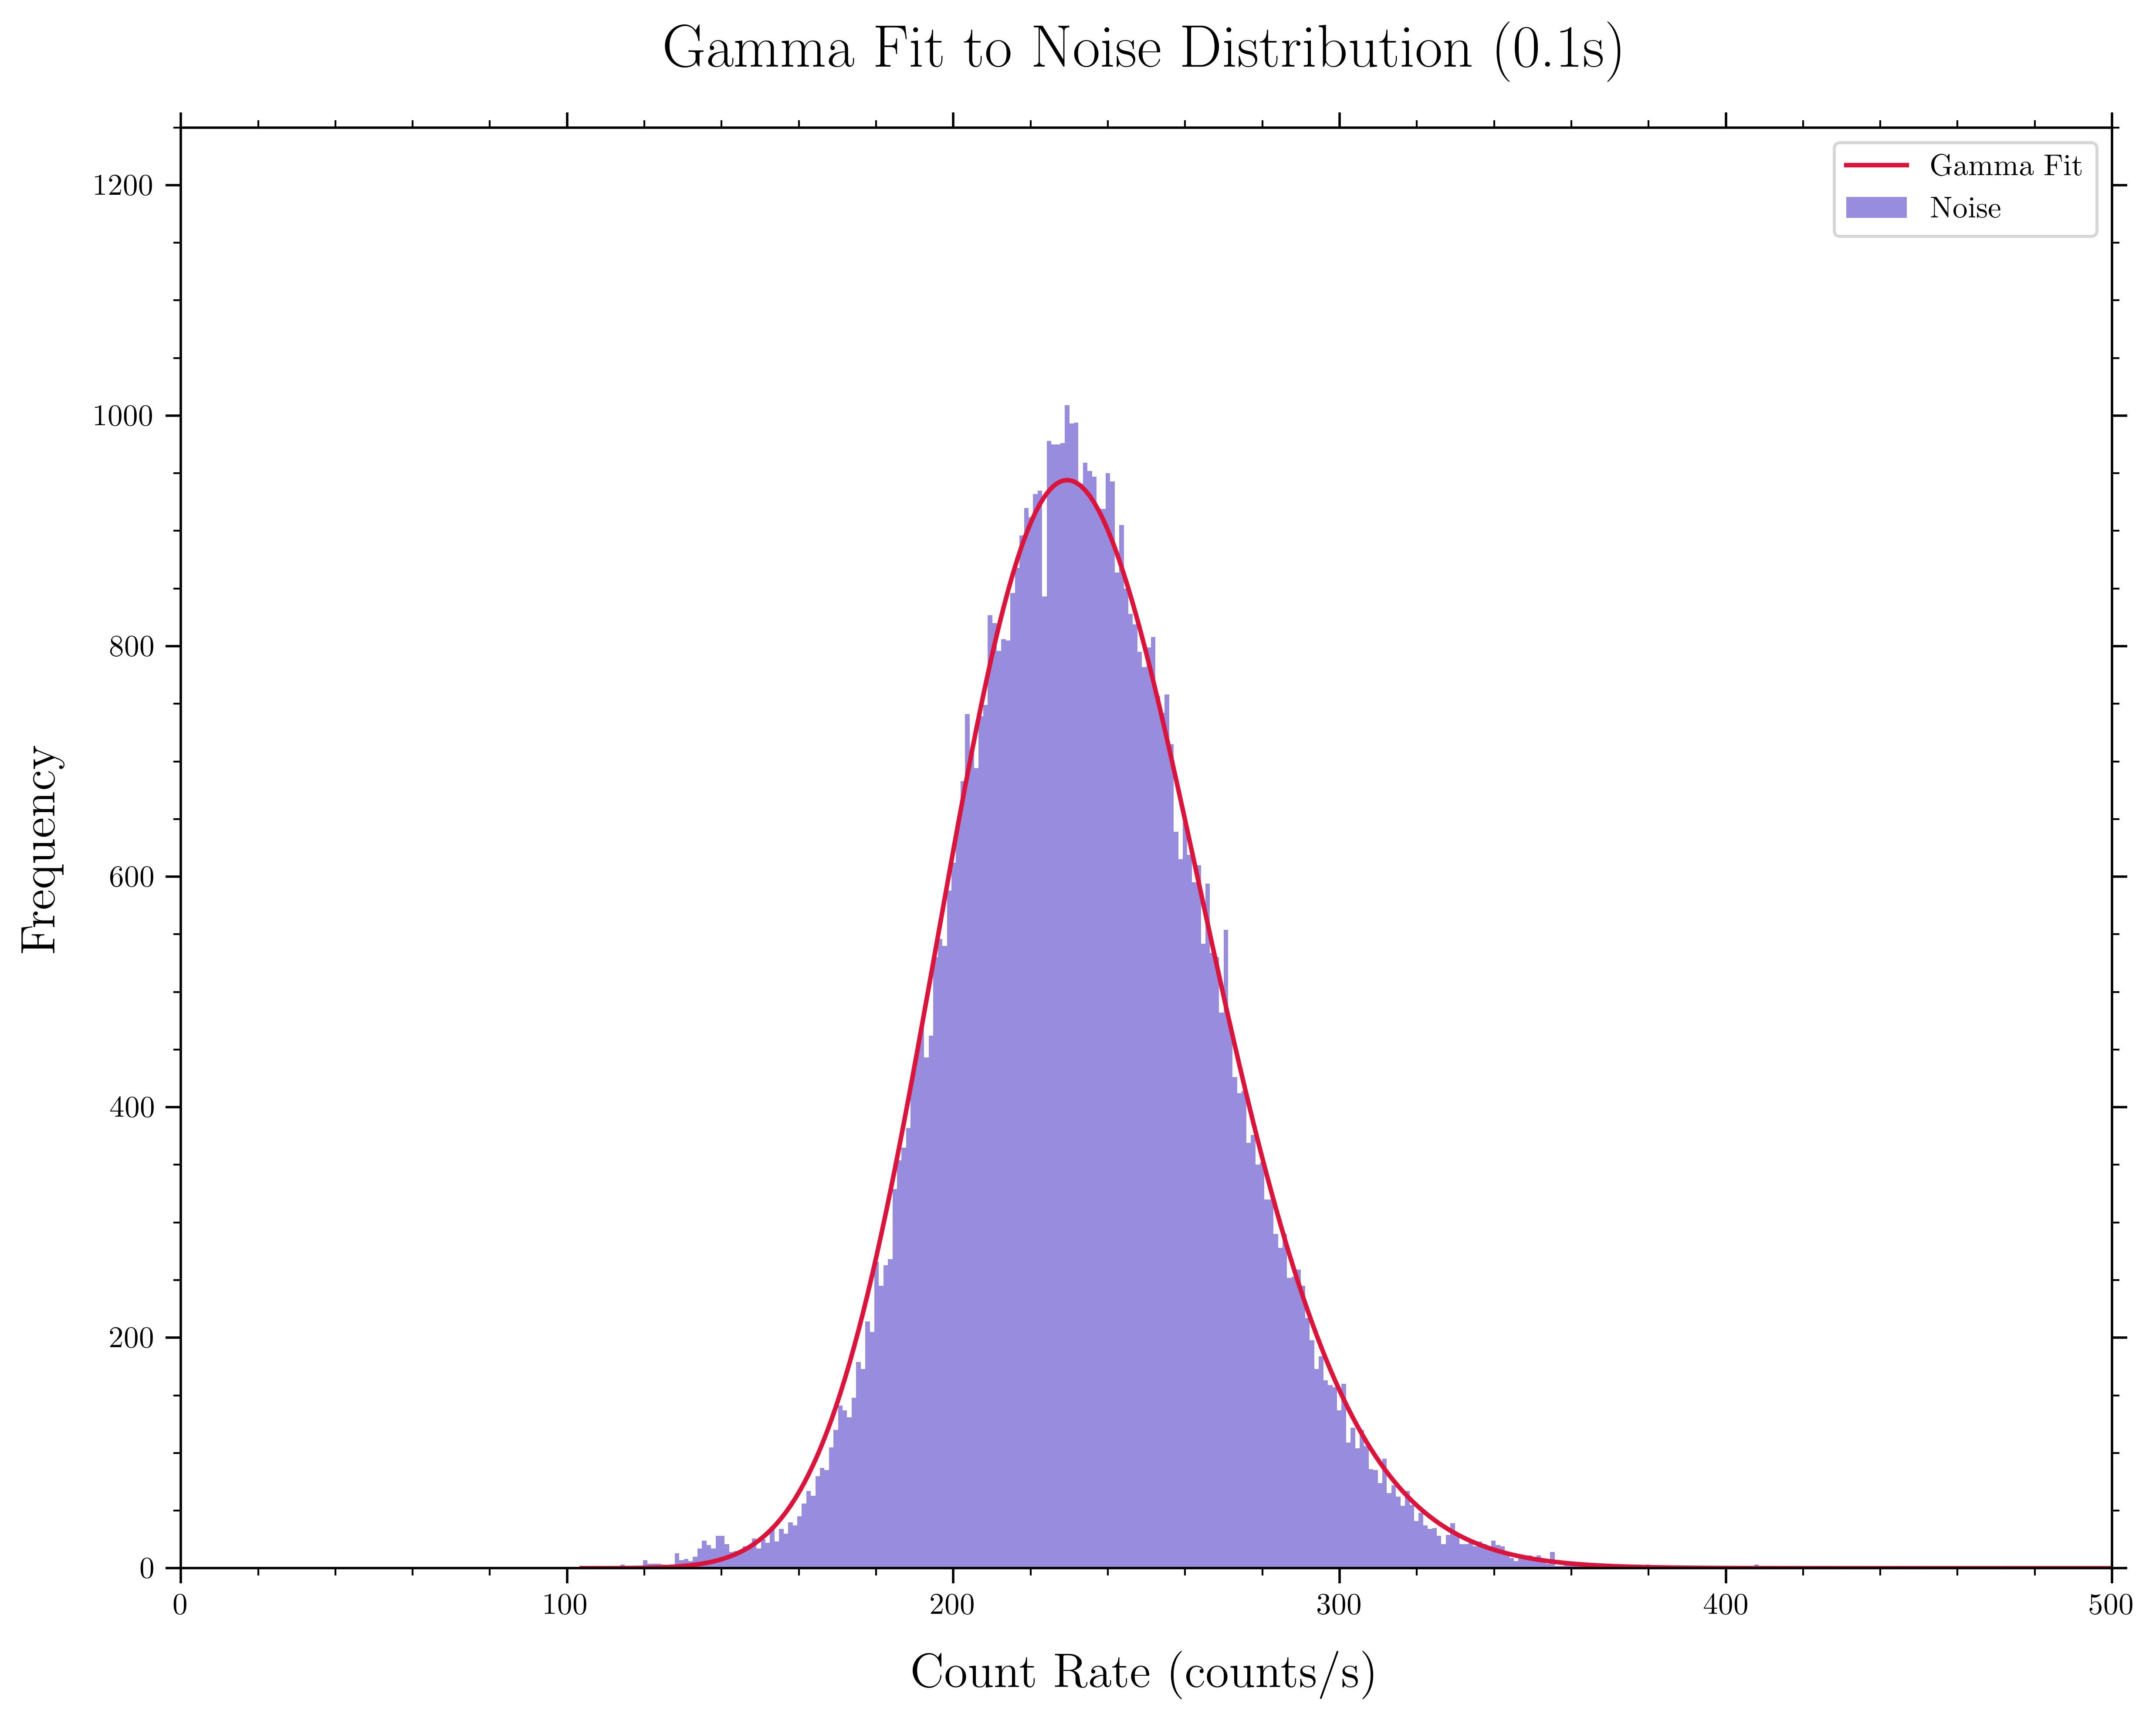
\includegraphics[width=0.8\textwidth]{Pictures/gamma_fit.png}
    \caption{Fitting a Gamma Distribution to the Noise (BinSize 0.1s) of Quadrant 0}
\end{figure}

We can see that the Gamma distribution is very close to the Poisson distribution in terms of the fit, maybe even better. We will quantify the fits in future sections.




%----------------------------------------------------------------------------------------
%	CHAPTER 4
%----------------------------------------------------------------------------------------


%----------------------------------------------------------------------------------------
%	BIBLIOGRAPHY
%----------------------------------------------------------------------------------------

% \label{References}
% \lhead{\emph{References}}
% \chapterimage{erosita_allsky} % Chapter heading image

% \chapter{Results and Discussion}

% \chapterimage{orion}

% \chapter{References}


%----------------------------------------------------------------------------------------
%	INDEX
%----------------------------------------------------------------------------------------

% \phantomsection
% \setlength{\columnsep}{0.75cm} % Space between the 2 columns of the index
% \printindex % Output the index

\end{document}

